    \documentclass[master, usehyperref, pdfmetadata]{finthesis}

\usepackage{graphicx}
\usepackage{booktabs}
\usepackage{float}
\usepackage{amsmath}
\usepackage{amssymb}
\usepackage{caption}
\usepackage{subcaption}
\usepackage{csquotes}
\sloppy

\addbibresource{references.bib}

\title{Forecasting Time-Varying Intermarket Dependencies Between Cryptocurrencies and Conventional Assets Using Machine Learning}
\author{Bogdan Babaev}
\date{2026-03-10}
\studid{TODO/2026}
\studprog{Мастер академске студије Електротехника и рачунарство}
\module{TODO: модул}
\course{Мастер рад}
\advisor{TODO: ментор}
\advisorfull{TODO: титула, име и презиме ментора}
\committee{TODO: члан комисије 1}
\committee{TODO: члан комисије 2}

% Задатак кандидата — приказује се на трећој насловној страни
\studentshould{истражи могућност прогнозирања временски-променљивих међутржишних зависности између криптовалута и конвенционалних финансијских актива применом модела машинског учења. У склопу тога кандидат треба да: (1) прикупи историјске дневне цене за Bitcoin и традиционалне активе (акцијски индекси, фондови племенитих метала, индекс америчког долара, Ethereum); (2) развије репродуцибилан рачунарски поступак за израчунавање временски-променљивих корелационих циљева помоћу клизних прозора и конструкцију предиктивних особина; (3) реализује ванузорачну евалуацију и поређење неколико модела машинског учења (AR, ElasticNet, Ridge, Random Forest, GBM, XGBoost) са DCC-GARCH(1,1) економетријским репером применом Diebold-Mariano теста; (4) уведе практични сигнални слој за рано детектовање стресних дана на тржишту традиционалних актива на основу динамике криптовалута и прогноза зависности.}

% Четврта насловна страна треба да садржи скенирану оверену пријаву мастер рада.
% Уколико пријава тренутно није доступна, коментаришите \fourthtitlepage у \maketitle:
\renewcommand{\maketitle}{%
    \firsttitlepage%
    \secondtitlepage%
    \thirdtitlepage%
%   \fourthtitlepage% <-- одкоментарисати када буде доступна скенирана пријава рада
}

\abstractsr{У овом мастер раду разматра се проблем прогнозирања променљивих међутржишних зависности између криптовалута и традиционалних финансијских актива. У фокусу је Bitcoin као основна криптовалута, док скуп традиционалних актива обухвата акцијске индексе, фондове везане за племените метале и индекс америчког долара. Развијен је репродуцибилан рачунарски поступак који покрива преузимање података, израчунавање логаритамских приноса, формирање временски променљивих корелационих циљева, конструисање особина, ванузорачну процену више модела машинског учења и поређење са DCC-GARCH економетријским репером. Поред основног задатка прогнозирања зависности, уведен је и практични слој за формирање раног сигнала ризика који треба да упозори инвеститора на стресне дане на тржишту традиционалних актива. Резултати показују да је временски променљива међутржишна зависност предвидива, али да највећи део предвидивости потиче из сопствене инерције циљне серије, док сложенији модели машинског учења доносе ограничено додатно побољшање у односу на једноставне ауторегресионе приступе. Практични сигнални слој даје умерене резултате и има смисла пре свега као додатни филтар ризика, а не као самосталан механизам за свакодневно одређивање смера тржишта.}
\keywordssr{криптовалуте, Bitcoin, међутржишне зависности, корелација, машинско учење, DCC-GARCH, управљање ризиком}

\abstracten{This thesis investigates whether information contained in cryptocurrency dynamics can be used to forecast time-varying dependency structures with conventional assets and, in a second step, to derive an early warning signal for investors. Bitcoin is treated as the base cryptocurrency, while the conventional asset universe includes equity indices, precious-metal exchange-traded funds, the U.S. dollar index, and Ethereum as an additional crypto reference. A reproducible machine-learning pipeline is developed for data acquisition, return construction, rolling-correlation target generation, feature engineering, walk-forward model evaluation, and benchmarking against a leakage-safe DCC-GARCH specification. The empirical results show that intermarket dependency is forecastable, but that most predictive power originates from persistence in the dependency series itself. Consequently, simple autoregressive baselines outperform more complex models on average, while machine-learning models still provide useful improvements relative to the DCC-GARCH benchmark. An investor-oriented signal layer based on crypto features and dependency forecasts achieves moderate but meaningful performance and is best interpreted as a risk-management overlay rather than a standalone market-timing engine.}
\keywordsen{cryptocurrencies, Bitcoin, intermarket dependency, correlation, machine learning, DCC-GARCH, forecasting, risk management}

\begin{document}

\maketitle
\makeabstract
\selectlanguage{english}
\tableofcontents
\listoffigures
\listoftables

\section{Introduction}

The integration of cryptocurrency markets into the broader financial system has transformed them from a fringe technological curiosity into a meaningful component of global risk transmission. Bitcoin in particular has become a continuously traded, highly visible, sentiment-sensitive asset whose price dynamics are monitored not only by crypto-native investors but also by portfolio managers, macro traders, and policy observers. As the market matures, an increasingly important research question emerges: can information extracted from cryptocurrencies reveal something useful about future conditions in conventional markets such as equities, metals, or currency-related instruments?

This thesis addresses that question by focusing on \emph{time-varying intermarket dependency}. Instead of attempting to forecast price levels directly, the thesis models the changing relationship between Bitcoin and conventional assets through rolling correlation structures. This distinction is important. Correlation is not constant over time, especially in periods characterized by liquidity shocks, inflation scares, monetary tightening, or abrupt shifts in investor risk appetite. When such shifts occur, the strength and sign of cross-market linkages may change faster than conventional long-horizon diversification assumptions would suggest.

The practical motivation of the thesis is equally important. A portfolio manager does not necessarily need a perfect one-day-ahead return forecast in order to make a useful decision. In many cases, what matters most is early recognition that the market environment is becoming unstable, that co-movements are changing, and that the probability of a stress episode in conventional assets is increasing. If cryptocurrency data can contribute to such early warning information, then even a moderate forecasting edge can have real value as a risk-management input.

The central research problem can therefore be stated in two layers. The first layer is methodological and scientific: are time-varying dependencies between Bitcoin and conventional assets forecastable in a disciplined out-of-sample framework, and how do machine-learning models compare with classical econometric benchmarks? The second layer is practical: can those dependency forecasts be translated into a market-relevant warning signal that helps an investor identify elevated downside risk in conventional markets more quickly?

To address these questions, the thesis constructs a reproducible forecasting pipeline in Python. The pipeline collects price data, transforms them into log returns, builds rolling-correlation targets using multiple window lengths, engineers lagged and volatility-based predictors, and evaluates a range of models in a walk-forward setting. The model set includes simple persistence benchmarks, regularized linear methods, tree-based ensemble methods, XGBoost, and a DCC-GARCH benchmark implemented in a leakage-safe way. On top of the dependency-forecasting layer, an investor-oriented signal layer is added to predict stress regimes for conventional assets on the basis of crypto-derived information and forecasted dependency dynamics.

The empirical findings point to a nuanced but useful conclusion. Dependency forecasting works. The problem is not random. However, the dominant source of predictability is persistence in the dependency process itself, meaning that the strongest baseline models are often autoregressive and naive persistence variants. This is not a weakness of the thesis; it is a substantive result. It implies that machine-learning value in this setting is more incremental and comparative than revolutionary. The second-layer signal model provides moderate predictive value, especially as an auxiliary risk filter, but does not support the claim that cryptocurrency data can perfectly predict the next direction of all conventional markets.

The contribution of the thesis is therefore threefold. First, it builds a clean, reproducible framework for forecasting rolling intermarket dependency between cryptocurrencies and conventional assets. Second, it provides a structured comparison between classical econometric modeling and machine-learning approaches under walk-forward evaluation. Third, it extends the analysis from dependency forecasting to an applied investor warning layer, thereby connecting the statistical problem to a practical decision-making use case.

The remainder of the thesis is organized as follows. Section 2 reviews the theoretical background of time-varying dependence, financial contagion, machine-learning forecasting, and model-comparison methodology. Section 3 presents the dataset, target construction, feature engineering, models, and evaluation framework. Section 4 reports the empirical results for dependency forecasting and the investor signal layer. Section 5 interprets the findings, clarifies what the results do and do not imply, and discusses limitations. Section 6 concludes and proposes directions for future research.

\section{Theoretical Background and Literature Review}

\subsection{Why intermarket dependency matters}

Intermarket dependency is one of the central concepts in modern finance because diversification benefits, contagion mechanisms, hedging decisions, and portfolio risk all depend on how assets move relative to one another. In the simplest textbook setting, dependence is often summarized by a constant correlation coefficient. In real markets, however, that assumption is too restrictive. Correlations are known to vary over time, to respond asymmetrically to shocks, and to strengthen precisely in those periods when diversification is most needed. This makes the forecasting of \emph{time-varying dependence} both theoretically meaningful and practically valuable.

The importance of dynamic dependence becomes even stronger when one of the markets under consideration is cryptocurrency-based. Bitcoin trades continuously, reacts rapidly to shifts in sentiment and liquidity, and is influenced by a wide range of narratives: inflation hedging, speculative demand, technological optimism, regulatory concerns, and global macro uncertainty. Because of that hybrid nature, Bitcoin can behave at different times like a speculative growth asset, a high-beta liquidity proxy, or a market-specific sentiment barometer. That shifting role makes its relationship with conventional assets especially suitable for a time-varying approach.

\subsection{Cryptocurrencies and conventional assets}

The literature on cryptocurrencies and conventional assets has developed along several lines. One strand studies Bitcoin as a standalone asset class and examines its return distribution, volatility clustering, tail risk, and weak-form efficiency. Another strand focuses on portfolio diversification and asks whether Bitcoin provides diversification benefits relative to equities, gold, oil, or fiat currencies. A third strand investigates connectedness, contagion, and spillovers across markets, especially during crisis periods.

A recurring theme in this literature is instability. The relationship between Bitcoin and stock indices, for example, tends to be weak or inconsistent in quiet periods but can strengthen during episodes of broad risk-on or risk-off positioning. Gold-related instruments, by contrast, may exhibit lower and more erratic dependence with Bitcoin, reflecting their different investor bases and different roles in multi-asset portfolios. Currency-related instruments such as the U.S. dollar index introduce another dimension because they proxy global liquidity conditions and defensive positioning.

These observations motivate the modeling choice adopted in this thesis. Rather than imposing a static relationship or fitting a single full-sample coefficient, the thesis models dependence as a moving object. This allows the analysis to capture gradual changes, abrupt regime shifts, and differences across window lengths.

\subsection{Rolling correlation as a forecasting target}

A rolling correlation is conceptually simple and empirically useful. At each point in time, the analyst computes the correlation between two return series over the most recent window of length $w$. By repeating this through time, one obtains a new series that summarizes the evolution of intermarket co-movement.

Using rolling correlation as a target has several advantages. First, it is directly interpretable. A positive value indicates co-movement in the same direction, whereas a negative value suggests a hedge-like relationship. Second, it is simple enough to be compared across assets and window lengths. Third, it allows the researcher to focus on changes in market structure rather than changes in price level alone.

At the same time, rolling correlation introduces methodological challenges. Because the target is already a smoothed function of recent returns, it is often highly persistent. That persistence may dominate predictive performance and make it difficult for more complex models to outperform simple autoregressive benchmarks. The thesis explicitly embraces this challenge rather than treating it as an inconvenience. If the dependency process is mainly predictable because it is persistent, then that fact itself is an important empirical result.

To stabilize the target and reduce boundary effects, the thesis applies the Fisher transform to the rolling correlation series. This step is common when dealing with correlation-like quantities because it maps bounded correlation values into an unbounded space that is often easier to model statistically.

\subsection{Econometric benchmark: DCC-GARCH}

A classical approach to dynamic dependence is the Dynamic Conditional Correlation Generalized Autoregressive Conditional Heteroskedasticity model proposed by Engle \cite{engle2002}. The DCC-GARCH framework separates the modeling of conditional volatility from the modeling of dynamic conditional correlation. In practical terms, each return series is assigned its own univariate GARCH-type process, while the correlation matrix evolves through time according to a dynamic updating equation.

DCC-GARCH is attractive because it is grounded in financial econometrics, explicitly accounts for heteroskedasticity, and has become a standard benchmark for studies of dynamic dependence. It is also especially relevant in this thesis because the target of interest is not merely volatility, but the relationship between two markets under changing variance conditions.

Nevertheless, DCC-GARCH is not guaranteed to dominate more flexible alternatives. It relies on a specific parametric structure and may struggle when the data exhibit nonlinear interactions or when the researcher is interested in short-horizon point forecasting of a smoothed target rather than full conditional covariance modeling. Moreover, naive implementations can inadvertently use future information if the model is fit over the full sample and only then compared to out-of-sample targets. For that reason, this thesis uses a leakage-safe walk-forward implementation of the DCC benchmark.

\subsection{Machine-learning approaches to forecasting}

Machine learning is useful in financial forecasting not because it automatically guarantees better performance, but because it provides a family of models capable of representing nonlinear patterns, threshold effects, and interactions among predictors. In this thesis, machine-learning methods are evaluated against both DCC-GARCH and simple persistence benchmarks.

\subsubsection{Regularized linear models}

Regularized linear models such as Ridge regression and Elastic Net are often strong baselines in structured tabular forecasting problems. Ridge regression shrinks coefficients to reduce variance, while Elastic Net combines shrinkage and variable selection through a mixture of L1 and L2 penalties \cite{zou2005}. These models are especially useful when features are correlated, as is often the case with lagged financial variables, rolling volatility measures, and multiple transformations of related return series.

Although linear in form, regularized models can remain competitive when the target is smooth and persistence-driven. In many real-world financial settings, such models perform well not because the underlying market is truly linear, but because the signal-to-noise ratio is limited and aggressive nonlinear fitting leads to overfitting.

\subsubsection{Tree-based ensemble models}

Random Forests aggregate many decision trees trained on bootstrapped samples and random feature subsets, reducing variance and improving robustness \cite{breiman2001}. Gradient Boosting Machines build trees sequentially so that each new tree focuses on residual errors made by the previous ensemble \cite{friedman2001}. XGBoost refines this boosting framework with regularization, optimized tree construction, and computational efficiency \cite{chen2016}.

These models are natural candidates for the present thesis because the relation between crypto-derived information and dynamic dependence may involve nonlinearities. For example, the effect of Bitcoin volatility on future equity dependence may differ depending on whether the market is already in a high-correlation regime. Tree ensembles are capable of detecting such interaction-like behavior without requiring the analyst to pre-specify it parametrically.

At the same time, tree-based models are not always favored in one-step-ahead forecasting of a smoothed target. If the target is overwhelmingly governed by its own lag, more flexible models may gain little while paying a variance penalty. This is one reason why a disciplined out-of-sample comparison is essential.

\subsection{Walk-forward evaluation and information leakage}

Financial time series require special care in evaluation. Random train-test splits are inappropriate because they destroy temporal order and create implicit look-ahead bias. The only credible way to compare models in a forecasting context is to ensure that every prediction uses only information available up to the forecast origin.

For that reason, this thesis uses a walk-forward procedure. At each step, models are fit on an expanding historical sample, predictions are produced for the next observation, and the process moves forward through time. Refitting is performed periodically rather than at every single point in order to balance realism and computational cost.

This evaluation design matters as much as model selection itself. A sophisticated model estimated with leakage can easily appear better than a simpler but properly evaluated competitor. Since one of the goals of the thesis is to provide a defensible empirical result, methodological discipline is treated as a first-class requirement.

\subsection{Model comparison and the Diebold--Mariano test}

When multiple forecasting models are available, simple ranking by average error is informative but not sufficient. A difference in RMSE or MAE does not automatically imply a statistically meaningful performance gap. The Diebold--Mariano test addresses this issue by comparing the loss differential of two forecast series under the null hypothesis of equal predictive accuracy \cite{diebold1995}.

In the context of this thesis, the DM test plays two roles. First, it clarifies whether the strongest machine-learning configuration materially outperforms the DCC-GARCH benchmark. Second, it helps determine whether any apparent machine-learning advantage remains meaningful once compared to simple autoregressive or naive persistence baselines.

This distinction is crucial for interpretation. Outperforming DCC-GARCH may justify the claim that flexible prediction methods add value relative to a classical benchmark. Failing to outperform a simple AR(1) baseline, however, would indicate that most forecastability is due to serial dependence in the target itself rather than rich cross-feature learning.

\subsection{From dependency forecasting to investor signaling}

A thesis focused purely on forecasting rolling correlation would already have a valid academic contribution. However, the practical motivation behind the present study requires an additional step. If investors are to benefit from crypto-derived information, that information must be translated into a decision-relevant object.

This is why the thesis introduces a second layer: an investor warning signal. Instead of asking whether the next-day return of a conventional asset will be positive or negative in a simplistic sense, the signal layer asks whether the next day is likely to belong to a \emph{stress regime}. This formulation is better aligned with the practical problem of risk reduction. Investors do not need a perfect classifier of every daily move; they need a timely warning that the environment is deteriorating.

The move from dependency forecasting to stress signaling also reflects a broader methodological insight. A model that is scientifically useful may not be directly tradable, and a model that is directly tradable may fail to explain much. By separating the two tasks, the thesis creates a transparent bridge between academic forecasting and applied portfolio risk management.

\subsection{Positioning of the present thesis}

The present thesis is positioned at the intersection of financial econometrics, machine learning, and applied risk analysis. It does not claim that cryptocurrency data alone can solve market timing. Instead, it examines a more defensible and intellectually coherent claim: that cryptocurrency dynamics contain information about changing intermarket dependencies, and that these dependency forecasts can be used to derive a modest but meaningful early warning signal for conventional markets.

This positioning matters for the final interpretation. The strongest contribution of the thesis lies in the forecastability of dynamic dependence and in the careful comparison between persistence baselines, machine-learning models, and a DCC-GARCH benchmark. The investor signal layer extends that contribution into a practical direction without overstating what the empirical evidence can support.

\section{Methodology}

\subsection{Research design}

The thesis adopts a layered research design. The first layer is a regression-style forecasting problem in which the target is the next value of a transformed rolling correlation series between Bitcoin and another asset. The second layer is a classification-style problem in which the output of the first layer, together with crypto-derived features, is used to estimate the probability of a stress day for the conventional asset. This structure mirrors the distinction between scientific measurement and practical action.

The design is intentionally conservative. Rather than optimizing purely for in-sample fit, all important modeling decisions are embedded in a walk-forward evaluation framework. This includes target formation, feature alignment, benchmark estimation, and signal generation. The objective is to preserve temporal realism and minimize the risk of accidental look-ahead bias.

\subsection{Asset universe and data source}

The empirical analysis uses daily market data obtained through the \texttt{yfinance} interface \cite{yfinance2026}. Bitcoin, represented by \texttt{BTC-USD}, serves as the base cryptocurrency throughout the study. The comparison set includes the following assets:

\begin{table}[H]
    \centering
    \caption{Asset universe used in the thesis.}
    \label{tab:asset_universe}
    \begin{tabular}{ll}
        \toprule
        Ticker & Interpretation \\
        \midrule
        \texttt{BTC-USD} & Bitcoin, base cryptocurrency \\
        \texttt{ETH-USD} & Ethereum, crypto reference asset \\
        \texttt{\^{}GSPC} & S\&P 500 index \\
        \texttt{\^{}IXIC} & NASDAQ Composite index \\
        \texttt{GLD} & Gold ETF \\
        \texttt{SLV} & Silver ETF \\
        \texttt{UUP} & U.S. Dollar Index ETF proxy \\
        \bottomrule
    \end{tabular}
\end{table}

This universe was chosen for substantive rather than purely technical reasons. The two equity indices represent broad U.S. risk assets. Gold and silver ETFs capture precious-metal exposure, often linked to inflation concerns, safe-haven narratives, or commodity sentiment. The dollar index proxy reflects global dollar strength and defensive macro positioning. Ethereum is included as an additional crypto benchmark in order to contrast cross-crypto dependency with crypto-to-conventional dependency.

\subsection{Return construction and preprocessing}

All price series are converted into daily log returns. Log returns are preferred because they are additive over time and are standard in both econometric modeling and machine-learning pipelines for financial time series. Missing observations are handled through alignment across available dates, and all downstream targets and features are built only after the return matrix is synchronized.

A cache-aware preprocessing workflow is used in the codebase. If raw price data already exist, they are reused to guarantee reproducibility. If the structure of prices or the ticker universe changes, the processed returns are recomputed. This avoids stale intermediary files while keeping the workflow efficient.

\subsection{Target construction: rolling dependency}

For each pair consisting of Bitcoin and another asset, a rolling correlation series is computed over windows of 14, 30, 60, and 90 trading days. Let $r_t^{(b)}$ denote the return of Bitcoin and $r_t^{(a)}$ the return of the other asset. For a given window length $w$, the dependency target at time $t$ is
\[
\rho_t^{(w)} = \text{corr}(r_{t-w+1:t}^{(b)}, r_{t-w+1:t}^{(a)}).
\]

The resulting series is then transformed using the Fisher transformation
\[
z_t^{(w)} = \frac{1}{2}\log\left(\frac{1 + \rho_t^{(w)}}{1 - \rho_t^{(w)}}\right),
\]
which maps the bounded correlation domain into an unbounded real-valued space. In the empirical implementation, the one-step-ahead value of the transformed dependency series is used as the main forecasting target.

A key implication of this design is that the target is already a smooth object. It is therefore much more persistent than a raw return series. This persistence is one of the defining empirical features of the thesis and is directly reflected in the later results.

\subsection{Feature engineering}

The feature set is intentionally structured around interpretable financial quantities. The goal is not to create an excessively large black-box predictor matrix, but to engineer a compact set of variables that can plausibly affect future dependency dynamics.

The features fall into several groups:

\begin{table}[H]
    \centering
    \caption{Main groups of predictors used in the dependency-forecasting layer.}
    \label{tab:feature_groups}
    \begin{tabular}{ll}
        \toprule
        Group & Description \\
        \midrule
        Dependency lags & Recent values of the rolling dependency target \\
        Return lags & Lagged returns of Bitcoin and the paired asset \\
        Rolling means & Local average return over short windows \\
        Rolling volatility & Local standard deviation of returns \\
        Spread features & Absolute and signed gaps between crypto and asset behavior \\
        Interaction-like structure & Implicitly captured by tree-based models \\
        \bottomrule
    \end{tabular}
\end{table}

Dependency lags are especially important because the target is persistent by construction. Return lags allow the models to react to recent directional information. Rolling means and volatility measures summarize local regime conditions. Spread-style features capture whether Bitcoin is currently moving more aggressively than the paired asset and whether that divergence might precede a change in dependency.

The investor signal layer inherits the best dependency forecast available for the pair and combines it with crypto-derived predictors to form a smaller classification-oriented feature set. In practice, this means that the second layer is informed by both the current crypto state and the estimated direction of the dependency process.

\subsection{Forecasting models}

\subsubsection{Baseline models}

Two simple baselines are included in every forecasting experiment. The first is \texttt{Naive\_Last}, which predicts the next dependency value using the most recent observed dependency. The second is \texttt{AR1}, which estimates a one-lag autoregressive structure. These baselines are essential because the target is persistent. Any more complex model must therefore justify itself relative to these very strong simple alternatives.

\subsubsection{Regularized linear models}

The linear machine-learning block includes Ridge and Elastic Net. Standardization is applied before fitting these models, since coefficient regularization depends on feature scaling. Ridge is expected to perform well when many predictors are weak but correlated. Elastic Net is more aggressive and can be advantageous if only a subset of variables contains stable information.

\subsubsection{Tree ensembles}

The non-linear block includes Random Forest, Gradient Boosting, and XGBoost. These models are fit in a walk-forward setting with periodic refits. In the implementation, XGBoost attempts GPU execution when available, but automatically falls back to CPU mode if the environment does not support the requested configuration. This makes the pipeline more robust and prevents a hardware-specific failure from invalidating the experiment.

\subsubsection{DCC-GARCH benchmark}

A leakage-safe DCC-GARCH walk-forward benchmark is implemented as a separate module in the project. This is a key methodological correction relative to many simplified comparisons found in exploratory work. Instead of fitting DCC over the full sample and then evaluating it as if it were out of sample, the benchmark is repeatedly re-estimated on the training window only, and forecasts are produced forward from that point. This makes the benchmark slower, but methodologically consistent.

\subsection{Investor signal layer}

The signal layer reframes the problem as an early warning classification task. The target is not generic next-day direction, but a \emph{stress day} indicator for the conventional asset. A stress day is defined relative to the distribution of negative returns, using a configurable sigma-based threshold. This target design is intentionally conservative and aligns better with the practical goal of downside protection.

Three classifiers are evaluated in this layer: logistic regression, random-forest classification, and gradient-boosted classification. The probability output of each model is compared with a threshold to decide whether the investor should treat the next day as elevated-risk. This makes the output interpretable as a probability-guided warning rather than a binary black-box trade instruction.

\subsection{Walk-forward estimation framework}

All experiments use an expanding-window walk-forward design. Let the initial estimation sample contain the first $T_0$ observations. For each forecast origin $t \geq T_0$, the model is fit using observations up to time $t$, then used to produce a prediction for $t+1$. The process continues until the end of the sample. Periodic refitting is used to reduce computational burden while preserving causal ordering.

This design has several benefits. It mirrors real forecasting conditions, supports fair benchmark comparisons, and generates a full time series of out-of-sample prediction errors. The latter is useful not only for average metrics, but also for rolling error diagnostics and Diebold--Mariano testing.

\subsection{Evaluation metrics}

For the dependency-forecasting layer, performance is evaluated using mean absolute error (MAE), root mean squared error (RMSE), and the out-of-sample coefficient of determination $R^2$. RMSE is emphasized in model ranking because it penalizes large deviations more strongly and is well suited to smooth continuous targets.

For the investor signal layer, the primary metrics are Balanced Accuracy, F1 score for the downside class, area under the ROC curve (AUC), and exit rate. Balanced Accuracy is especially important because stress-day classification is an imbalanced problem. F1 for the downside class focuses attention on the quality of negative-event detection. Exit rate measures how often the signal would remove the investor from the market, thereby connecting prediction quality with practical usage frequency.

\subsection{Model comparison methodology}

Average metrics alone can be misleading when model differences are small. The thesis therefore applies the Diebold--Mariano test to compare forecast loss series between selected model pairs. The main comparison of interest is between the strongest non-benchmark machine-learning model and the DCC-GARCH benchmark. A secondary comparison contrasts that machine-learning model with the naive persistence baseline.

This setup is intentionally transparent. The thesis does not hide the fact that the best overall model may be a simple baseline. Instead, the DM framework is used to distinguish between three levels of claim:

\begin{enumerate}
    \item whether dependency is forecastable at all,
    \item whether machine learning improves upon a classical econometric benchmark,
    \item whether machine learning adds value beyond persistence.
\end{enumerate}

The empirical conclusions of the thesis are organized around precisely these three levels.

\subsection{Implementation and reproducibility}

The entire workflow is implemented in Python and organized as a modular codebase. The main pipeline coordinates loading configuration files, computing returns, generating targets, building features, fitting models, producing prediction files, saving figures, and exporting LaTeX-ready tables. Dedicated modules are used for DCC walk-forward benchmarking, notebook support, and the investor signal layer. This modular structure is important because the thesis is not merely a conceptual study but a reproducible computational artifact.

Outputs are stored in a structured directory hierarchy. Metrics, DM tests, and signal results are saved as CSV files; thesis-ready tables are exported to LaTeX; and visual diagnostics are saved as figures. This design reduces manual post-processing and helps align the research workflow with the writing workflow.

\subsection{Methodological expectations}

Before turning to the empirical results, it is useful to clarify what would count as success. Success in this thesis does not mean discovering a model that perfectly predicts all conventional markets from Bitcoin. That would be an unrealistic standard for any serious financial forecasting study. A more appropriate standard is the following:

\begin{itemize}
    \item the dependency target should display out-of-sample forecastability,
    \item the benchmark comparison should reveal whether machine learning improves on DCC-GARCH,
    \item the investor signal layer should provide non-random and practically interpretable stress warnings.
\end{itemize}

These criteria are modest but scientifically defensible. They allow the thesis to make claims that are both empirically supported and intellectually honest.

\section{Empirical Results}

\subsection{Overview of the output set}

The final pipeline produces a complete set of empirical artifacts: out-of-sample metrics, model rankings, Diebold--Mariano comparisons, investor-signal statistics, prediction files, and thesis-ready figures. This matters because the contribution of the thesis is not limited to one isolated table. The project generates a consistent collection of results that can be inspected from several complementary angles: average forecast accuracy, statistical significance of differences, regime-specific diagnostics, and practical stress warnings.

At the broadest level, the results support the claim that the dependency process is forecastable. However, they also show that the forecasting problem is dominated by target persistence. This means that the thesis produces a scientifically meaningful result, but not a simplistic story in which the most complex model necessarily wins.

\subsection{Average dependency-forecasting performance}

Table~\ref{tab:model_ranking_summary} summarizes the average out-of-sample performance of the main models across all dependency experiments. The ranking is based primarily on RMSE.

\begin{table}[H]
    \centering
    \caption{Average forecasting performance across dependency experiments.}
    \label{tab:model_ranking_summary}
    \begin{tabular}{lrrr}
        \toprule
        Model & Average RMSE & Average MAE & Average $R^2$ \\
        \midrule
        AR1 & 0.0667 & 0.0405 & 0.9421 \\
        Naive\_Last & 0.0674 & 0.0396 & 0.9409 \\
        Ridge & 0.0916 & 0.0637 & 0.8914 \\
        ElasticNet & 0.0923 & 0.0644 & 0.8898 \\
        RF & 0.1013 & 0.0711 & 0.8687 \\
        GBM & 0.1038 & 0.0734 & 0.8622 \\
        XGB\_GPU & 0.1057 & 0.0758 & 0.8566 \\
        DCC\_GARCH & 0.2345 & 0.1848 & 0.2788 \\
        \bottomrule
    \end{tabular}
\end{table}

Several points are immediately visible. First, the best average model is not the most complex one but the AR1 baseline. Second, the naive persistence model is almost indistinguishable from AR1 in average RMSE. Third, regularized linear machine-learning models occupy a middle position and outperform tree ensembles on average. Fourth, DCC-GARCH is clearly weaker than all major alternatives in this dataset and evaluation setting.

The interpretation is straightforward but important. The dependency target is strongly persistent, and that persistence carries most of the predictive signal. This is why the simplest autoregressive structures dominate the ranking. A more complex model cannot gain much unless it extracts information beyond what is already contained in the lagged dependency itself.

\subsection{Representative forecast example}

Figure~\ref{fig:sp500_forecast} shows a representative out-of-sample forecast panel for the Bitcoin--S\&P 500 pair using the 30-day rolling window. This pair is substantively important because it links the cryptocurrency market to a broad benchmark of conventional equity risk.

\begin{figure}[H]
    \centering
    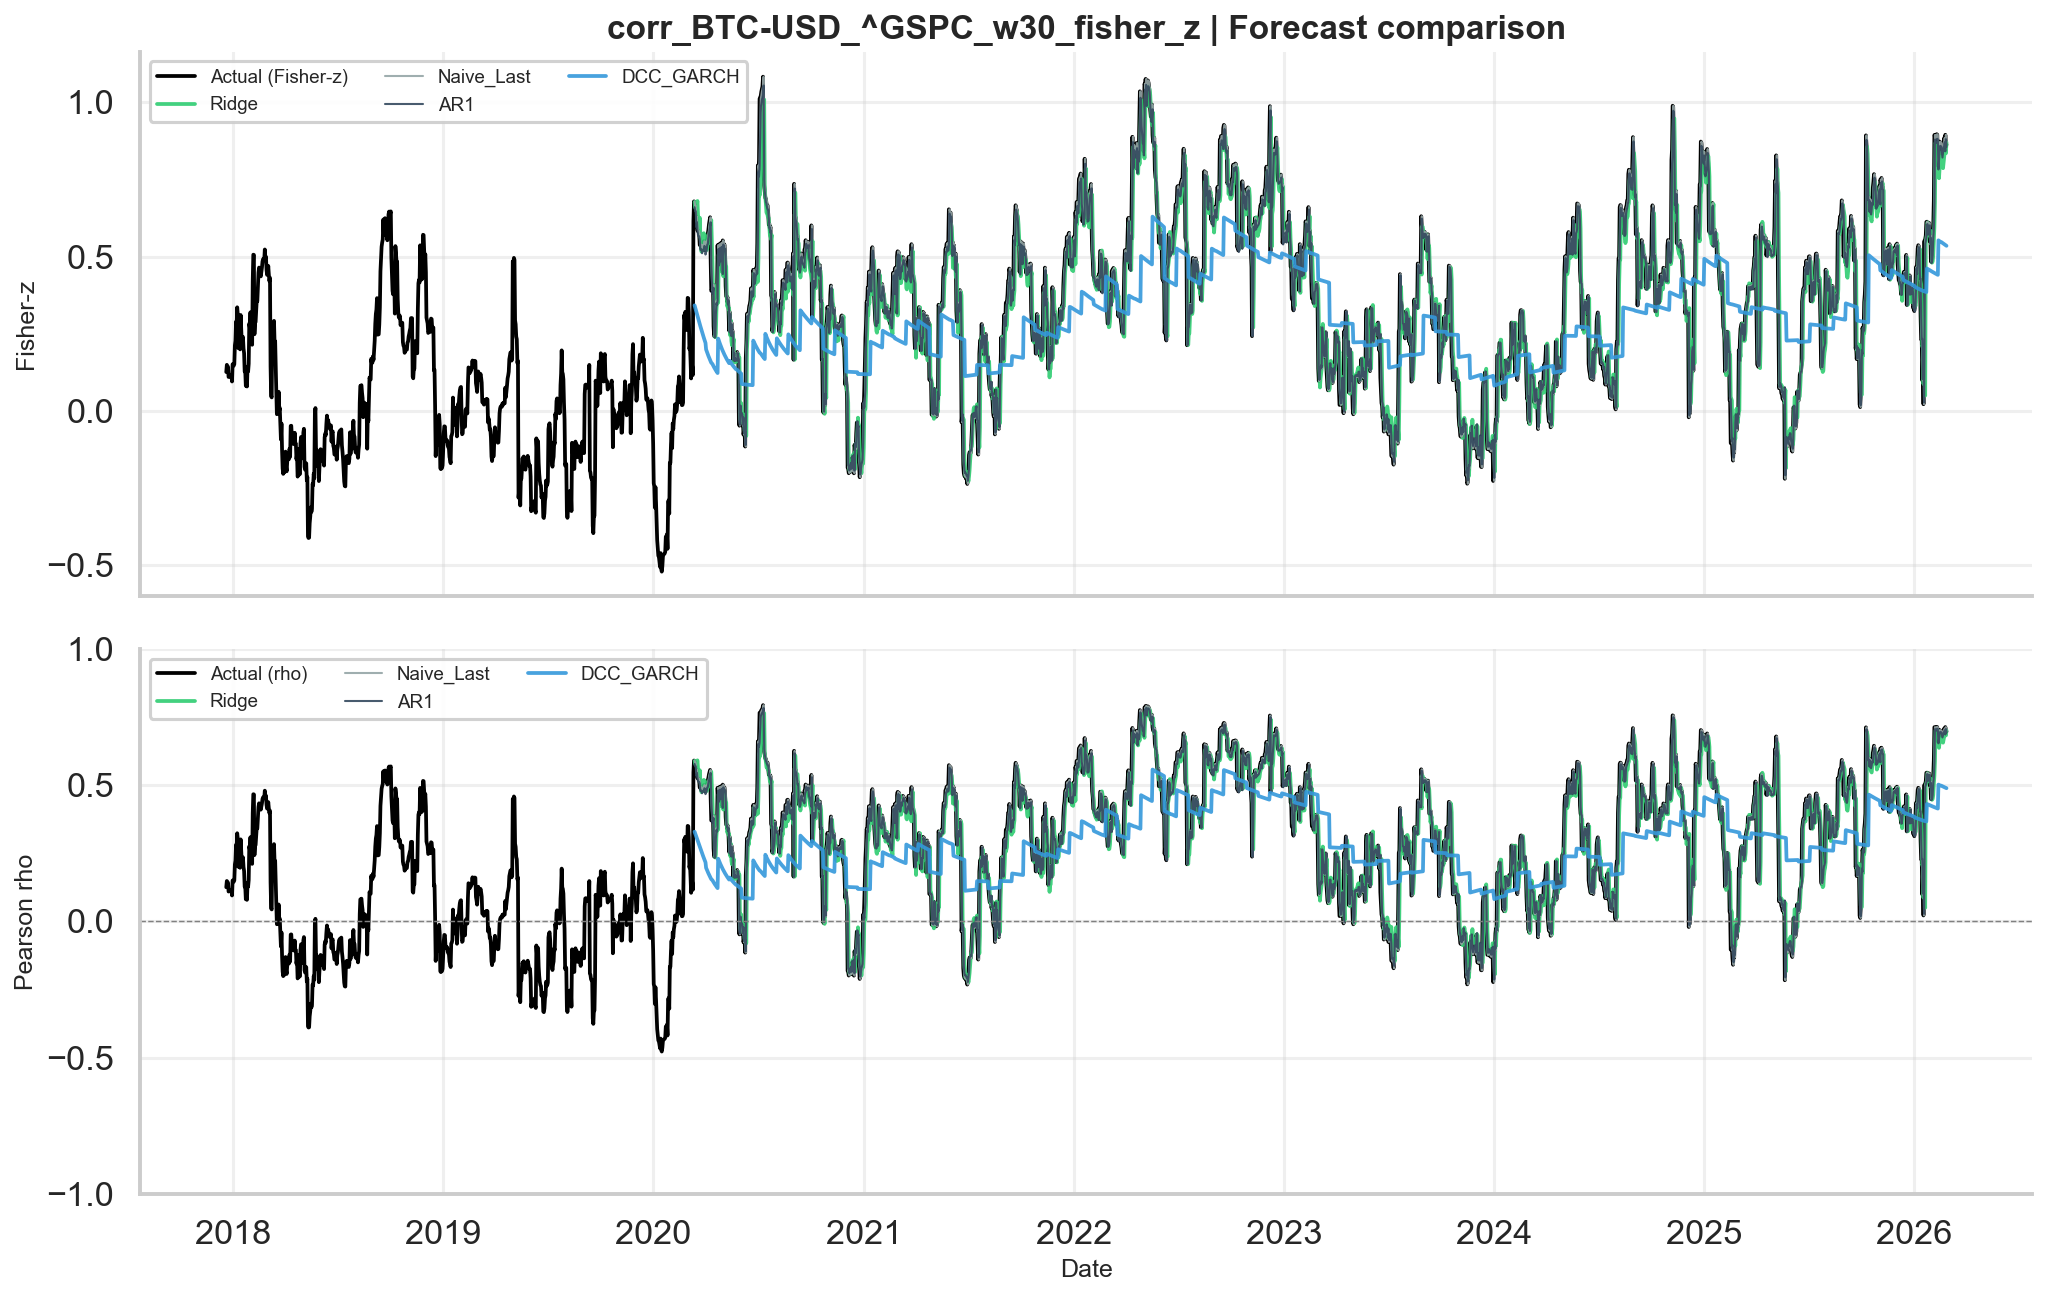
\includegraphics[width=0.95\textwidth]{../outputs/figures/thesis_forecast_corr_BTC-USD_^GSPC_w30_fisher_z.png}
    \caption{Observed and predicted dependency for the Bitcoin--S\&P 500 pair at the 30-day window.}
    \label{fig:sp500_forecast}
\end{figure}

The figure illustrates several characteristic features of the forecasting problem. First, the target moves in a relatively smooth manner, consistent with the use of rolling-correlation construction. Second, the strongest models track broad directional changes reasonably well. Third, local regime shifts remain difficult, particularly when the dependency process changes rapidly. This is exactly the type of environment in which a DCC benchmark may lag and where flexible machine-learning methods can sometimes provide a relative improvement even if they do not beat persistence baselines on average.

\subsection{Forecasting performance by asset class}

The average model ranking hides useful cross-asset variation. The BTC--ETH dependency tends to be the easiest to forecast because the two assets belong to the same broader market complex and often co-move strongly. This is reflected in very high out-of-sample $R^2$ values, especially for longer rolling windows, where the dependency target becomes even smoother.

Gold- and silver-related dependencies occupy an intermediate position. The rolling correlation between Bitcoin and gold or silver does exhibit structure, but it is less stable than the cross-crypto relation and may alternate between low, weakly positive, and weakly negative regimes. Even so, the experiments show that these targets remain forecastable and that persistence-based models are particularly strong.

The equity-index pairs, Bitcoin--S\&P 500 and Bitcoin--NASDAQ, are arguably the most relevant from a practical portfolio perspective. These relations matter because they connect crypto behavior with broad risk appetite. The results show that these dependencies are forecastable, but they also reveal substantial regime sensitivity. In some periods, the relation looks like a shared risk-on factor; in other periods, it weakens or reconfigures.

The dollar-index proxy pair has the weakest practical investor interpretation but remains analytically useful. It captures whether Bitcoin's dependency with a macro-defensive instrument is sufficiently structured to carry forecastable information. The answer is mixed but still informative.

\subsection{Why simple models dominate}

A central empirical finding of the thesis is that simple models dominate average performance. This does not invalidate the machine-learning approach. Instead, it clarifies the nature of the target. Because rolling dependency is a persistent, smoothed object, the one-step-ahead forecasting task is close to a persistence problem. Any complex model that attempts to outperform this baseline must learn subtle deviations from persistence rather than the bulk of the target dynamics.

This observation is reinforced by the feature-importance diagnostics from the Random Forest analysis. The lagged dependency term overwhelmingly dominates the ranking, while additional features such as local return volatility or return spreads contribute only marginally. In practical terms, the thesis shows that the problem is forecastable primarily because the target remembers its recent past.

\subsection{Comparison with DCC-GARCH}

Even though simple baselines dominate overall performance, machine learning remains useful in benchmark comparison. The DCC-GARCH model is a natural econometric reference point, but in this empirical setting it is not competitive on average. Figure~\ref{fig:dm_heatmap} presents a heatmap summary of the Diebold--Mariano comparison between a strong machine-learning candidate and the DCC benchmark.

\begin{figure}[H]
    \centering
    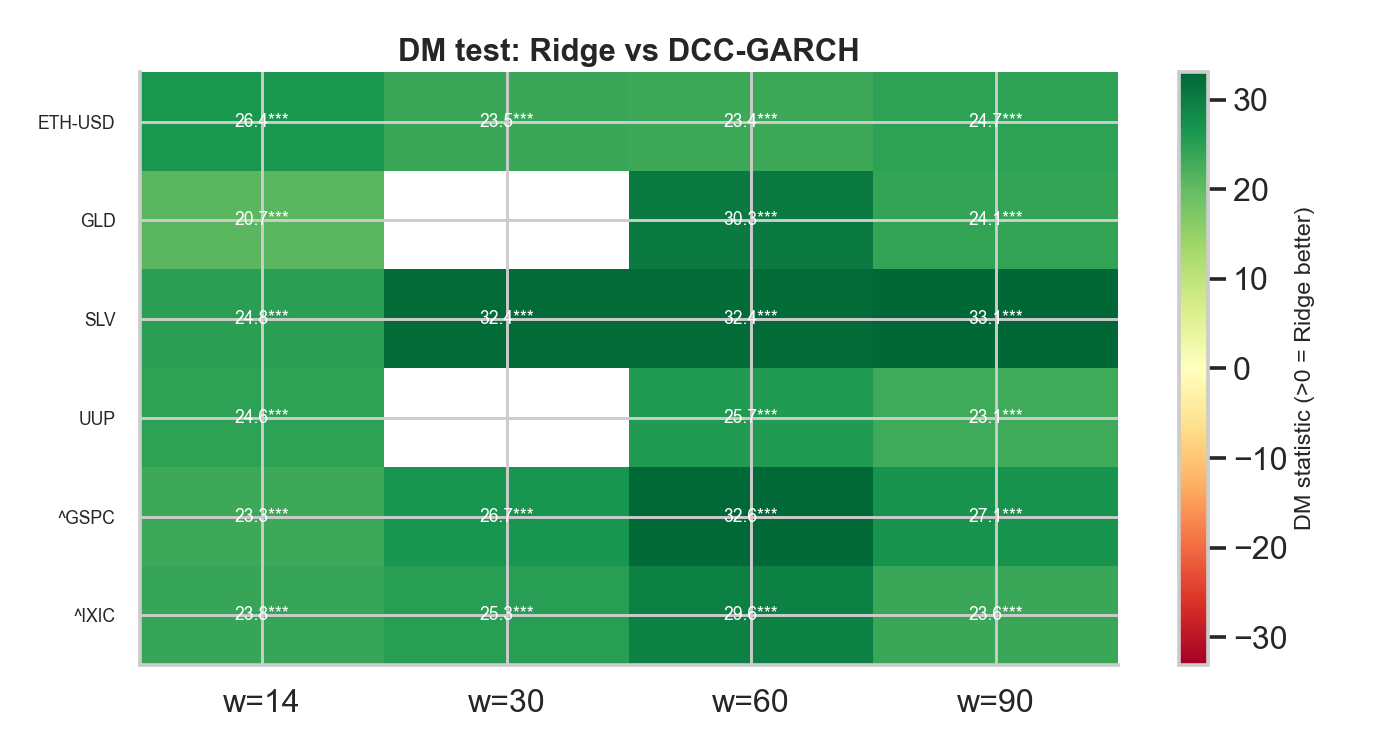
\includegraphics[width=0.82\textwidth]{../outputs/figures/dm_heatmap_Ridge_vs_DCC.png}
    \caption{Diebold--Mariano comparison against DCC-GARCH across dependency experiments.}
    \label{fig:dm_heatmap}
\end{figure}

The DM results support the claim that the strongest machine-learning model frequently outperforms DCC-GARCH in a statistically meaningful sense. This is an important result because it suggests that flexible predictive models can adapt more effectively than a classical conditional-correlation benchmark when the target is treated as a direct forecasting object.

At the same time, the DM analysis should not be overinterpreted. Beating DCC-GARCH does not imply beating persistence. The thesis therefore distinguishes clearly between \emph{benchmark superiority} and \emph{overall superiority}. Machine learning succeeds at the former more often than at the latter.

\subsection{Error-profile diagnostics}

Average error metrics summarize performance compactly, but they do not explain when models succeed or fail. The project therefore includes rolling RMSE diagnostics and forecast-error distribution plots. Figure~\ref{fig:rolling_rmse} illustrates how the error profile evolves through time for a representative experiment.

\begin{figure}[H]
    \centering
    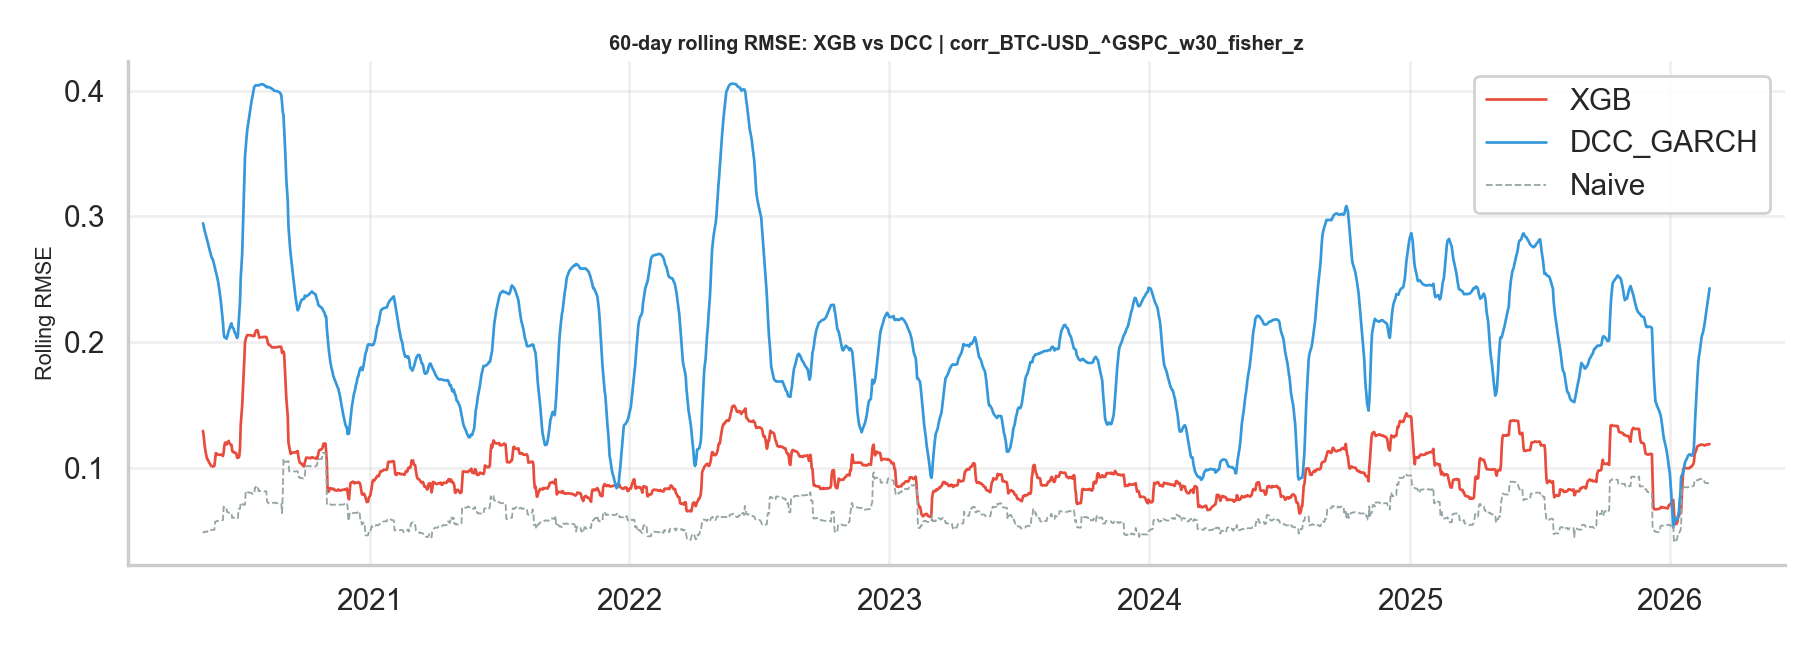
\includegraphics[width=0.9\textwidth]{../outputs/figures/rolling_rmse_corr_BTC-USD_^GSPC_w30_fisher_z.png}
    \caption{Rolling RMSE profile for the Bitcoin--S\&P 500 dependency forecast.}
    \label{fig:rolling_rmse}
\end{figure}

These diagnostics show that forecast quality is not constant through time. When the dependency process remains stable, even simple models perform well. When the market undergoes a regime transition, all models deteriorate, but the magnitude of the deterioration differs. This observation supports the practical value of model monitoring rather than one-off model selection.

The error-distribution and scatter diagnostics further show that the main challenge is not random noise alone but episodic underreaction to abrupt changes. In other words, the models tend to capture the low-frequency evolution of dependency better than the sharp turning points.

\subsection{Investor signal layer: average results}

The second empirical layer transforms crypto-derived information and dependency forecasts into a stress-warning problem. Table~\ref{tab:signal_summary} presents average classification results by model family.

\begin{table}[H]
    \centering
    \caption{Average investor-signal performance by classifier family.}
    \label{tab:signal_summary}
    \begin{tabular}{lrrr}
        \toprule
        Signal model & Balanced Accuracy & F1\_down & AUC \\
        \midrule
        Logit & 0.506 & 0.209 & 0.508 \\
        GBM\_Cls & 0.501 & 0.033 & 0.520 \\
        RF\_Cls & 0.500 & 0.030 & 0.519 \\
        \bottomrule
    \end{tabular}
\end{table}

The signal layer is deliberately more difficult than the first-layer regression problem. Stress-day detection is inherently noisy, class-imbalanced, and economically asymmetric. In this setting, the logistic model emerges as the most stable family. It does not produce spectacular scores, but it balances sensitivity and specificity better than the tree-based alternatives, which often collapse into extremely low exit rates and near-zero F1 for the downside class.

The correct interpretation is therefore moderate but positive. The signal layer is not strong enough to serve as a complete trading engine. However, it appears useful as a risk-management overlay, especially when applied to broad equity markets where avoiding a subset of stress periods may matter more than predicting every ordinary day.

\subsection{Best signal configurations}

The best single signal configurations occur for the S\&P 500 pair. In particular, the 30-day window combined with logistic classification reaches a Balanced Accuracy of 0.5405 and an F1 score of 0.2523 for the downside class. These values are not close to perfect prediction, but they are meaningfully above a purely random balanced baseline.

Figure~\ref{fig:signal_sp500} illustrates the signal output for the Bitcoin--S\&P 500 pair. The figure makes it easier to understand how the signal would be used in practice: not as a daily directional trade command, but as a warning indicator marking periods of elevated probability of stress.

\begin{figure}[H]
    \centering
    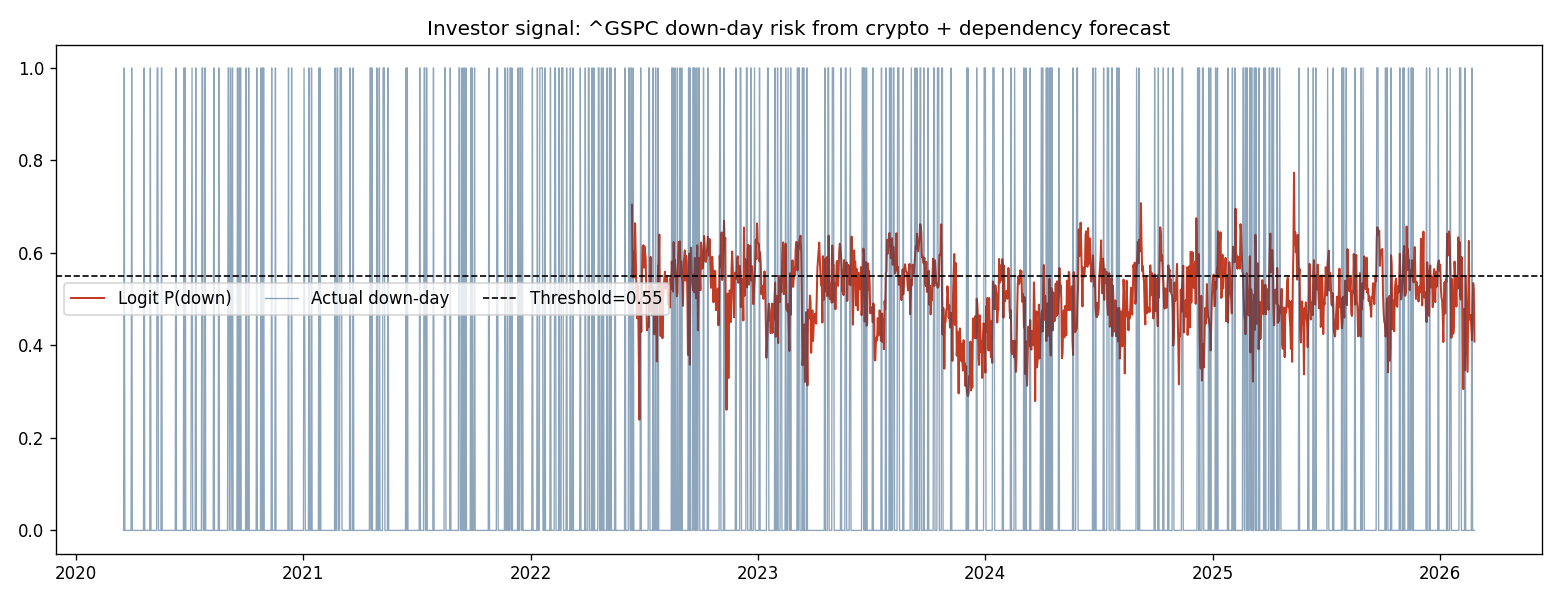
\includegraphics[width=0.95\textwidth]{../outputs/figures/signal_corr_BTC-USD_^GSPC_w30.png}
    \caption{Investor warning signal for stress days in the S\&P 500 market.}
    \label{fig:signal_sp500}
\end{figure}

For NASDAQ, metals, and the dollar proxy, the results are more mixed. This again suggests that the practical usefulness of the signal layer depends on market context. Equities appear more responsive to the kind of crypto-linked information captured by the feature set, whereas metal and currency proxies exhibit weaker and less stable signal behavior.

\subsection{Practical meaning of the signal layer}

A useful way to interpret the signal layer is through the question: what would a cautious investor do differently if the signal were available? The answer is not that the investor would trade every day. Rather, the signal would contribute to decisions about whether exposure should be reduced when market conditions become more fragile.

This practical framing aligns with the metrics reported in the project. Exit rate is an important complement to predictive accuracy because a model that almost never signals can look stable without being useful, while a model that signals too often may create excessive turnover. The logistic model occupies a middle ground that is more defensible from a portfolio-risk perspective.

\subsection{Sensitivity to window length}

Window length materially affects results. Short windows are more responsive but noisier; long windows are smoother but more inertial. This creates a trade-off between adaptability and stability. The experiments show that medium windows, especially 30 days, often provide a useful compromise. They preserve enough responsiveness to capture changing market structure while remaining smooth enough for stable one-step-ahead forecasting.

The sensitivity plots generated by the project also show that the apparent role of machine learning depends on this choice. With longer windows, persistence becomes even stronger and the relative advantage of complex models tends to diminish. This supports the broader thesis conclusion that the structure of the target itself largely determines the ranking of models.

\subsection{Summary of empirical findings}

The empirical results of the thesis can be summarized in four main statements:

\begin{enumerate}
    \item Time-varying dependency between Bitcoin and conventional assets is forecastable in an out-of-sample walk-forward setting.
    \item Most of the predictive power comes from persistence in the dependency process, which explains the strong performance of AR1 and naive baselines.
    \item Machine-learning models often outperform the DCC-GARCH benchmark, but usually do not outperform the strongest simple baselines on average.
    \item The investor signal layer delivers moderate, practically interpretable results and is best viewed as a risk-management aid rather than a standalone market-direction oracle.
\end{enumerate}

These results are coherent, internally consistent, and sufficient to support both the scientific and practical parts of the thesis. Their full interpretation is developed in the next section.

\section{Discussion}

\subsection{What the thesis demonstrates}

The strongest conclusion of the thesis is that time-varying intermarket dependency is not merely descriptive; it is forecastable. This matters because much of the literature treats rolling correlation primarily as an ex post diagnostic tool. In the present work, it becomes a genuine prediction target evaluated under strict temporal ordering. The empirical evidence shows that this target retains enough structure to support meaningful out-of-sample forecasting.

However, the thesis also demonstrates something equally important: forecastability does not automatically imply that highly flexible models dominate. In fact, the average ranking shows the opposite. The best performers are simple persistence-based models. This reveals a central property of the target itself. Because rolling dependency is constructed from overlapping windows and then Fisher-transformed, it behaves as a smooth, highly autocorrelated series. Any model that ignores this fact is likely to misunderstand the problem.

\subsection{Why the persistence result is valuable}

At first glance, it may seem disappointing that AR1 and Naive\_Last outperform the more complex alternatives. Yet this is a scientifically useful finding. A thesis does not become stronger by forcing machine learning to win at any cost. It becomes stronger by identifying the true source of predictability.

In this case, the evidence indicates that the main forecasting signal is embedded in the recent path of the dependency series itself. This has two implications. First, dependence processes between Bitcoin and conventional assets possess memory. Second, many sophisticated predictors add only marginal information beyond that memory, at least for the one-step-ahead horizon studied here.

This interpretation is also methodologically healthy. Financial forecasting often suffers from exaggerated claims driven by in-sample flexibility. The present thesis resists that temptation and shows that when the evaluation design is honest, simple baselines can remain formidable competitors.

\subsection{How machine learning still adds value}

The fact that simple baselines dominate average ranking does not mean that machine learning is irrelevant. Machine learning adds value in at least three ways.

First, it provides a broader comparison class, allowing the thesis to test whether nonlinear and interaction-capable methods can exploit information unavailable to linear persistence models. Second, even when these models do not win on average, they often improve upon the DCC-GARCH benchmark. Third, machine learning becomes more relevant in the second-layer signal problem, where the objective shifts from direct dependency forecasting to stress-warning classification.

This means the contribution of machine learning in the thesis is comparative and structural rather than purely top-ranked. The thesis demonstrates where machine learning helps, where it does not, and why.

\subsection{Interpretation of the DCC-GARCH result}

The relatively weak performance of DCC-GARCH deserves careful discussion. DCC is a respected econometric benchmark and remains conceptually appropriate for modeling dynamic covariance structures. Nevertheless, the empirical setup of this thesis places it in a demanding role: short-horizon direct forecasting of a smoothed target under walk-forward re-estimation.

Under those conditions, DCC-GARCH appears less competitive than expected. There are several possible reasons. The benchmark is parametric and therefore less flexible in responding to unusual local changes. The target of interest is not the entire covariance structure but a derived correlation-like quantity. Finally, the leakage-safe walk-forward implementation removes any accidental advantage that might arise from fitting the benchmark on the full sample.

This result should not be interpreted as a universal rejection of DCC-GARCH. Rather, it suggests that in the specific setting of one-step-ahead forecasting of rolling dependency between Bitcoin and conventional assets, DCC is a weaker forecasting engine than simpler persistence models and several machine-learning alternatives.

\subsection{Practical meaning for investors}

The investor motivation behind the thesis must be interpreted carefully. The empirical results do not support the claim that cryptocurrency data can reliably predict the exact next-day direction of all conventional markets. Such a claim would be too strong. What the thesis does support is a narrower and more defensible practical statement: cryptocurrency-derived information can contribute to an early warning system for elevated risk in conventional assets.

This is why the signal layer is framed as a \emph{risk overlay}. In practical portfolio terms, such a signal would not replace valuation, macro analysis, or strategic allocation. Instead, it could be used to increase caution, reduce exposure, or tighten risk limits when the probability of a stress regime becomes elevated.

For a real investor, this distinction is crucial. A moderate but interpretable warning signal can still be useful, especially when the cost of missing major downside episodes is large relative to the cost of occasional unnecessary caution.

\subsection{Why broad equities respond more clearly than some other assets}

The signal results are strongest for the S\&P 500 and somewhat weaker for NASDAQ, metals, and the dollar index proxy. This pattern is economically plausible. Broad equity markets are strongly tied to global risk appetite, liquidity conditions, and investor sentiment, all of which also influence Bitcoin. Precious metals and dollar-related instruments may react to a broader set of macro forces not fully captured by the crypto-centered feature set used in the thesis.

This suggests that the signal layer is most naturally interpreted as a crypto-informed risk indicator for growth-sensitive conventional markets rather than a universal warning engine across all asset classes.

\subsection{Methodological strengths of the thesis}

Several methodological choices strengthen the credibility of the empirical conclusions.

First, the pipeline is reproducible and modular. Second, the DCC benchmark is implemented in a leakage-safe manner rather than through a shortcut comparison. Third, all main models are evaluated in a walk-forward structure. Fourth, the thesis does not rely on a single metric but combines RMSE, MAE, $R^2$, Diebold--Mariano testing, Balanced Accuracy, F1, AUC, and exit-rate interpretation.

Together, these choices reduce the risk that the reported conclusions are artifacts of one particular model, one particular metric, or one particular coding shortcut. This is especially important for a thesis that aims to bridge methodological rigor and practical usefulness.

\subsection{Limitations}

The thesis also has important limitations that must be acknowledged openly.

The first limitation is frequency. All experiments are conducted on daily data. This is appropriate for a broad academic study and compatible with the chosen asset universe, but it may miss intraday information flow and very short-lived spillovers.

The second limitation is horizon. The core forecasting problem is one-step-ahead. This is a natural first design choice, yet it favors persistence-driven models and does not fully explore how predictive structure might evolve at multi-day or weekly horizons.

The third limitation is target design. Rolling correlation is interpretable and useful, but it is only one representation of dependency. Alternative dependence measures, such as tail dependence, copula-based measures, realized covariance, or dynamic partial correlations, could reveal additional structure.

The fourth limitation concerns the signal layer. The stress target is economically sensible, but still relatively simple. Different definitions of stress, including drawdown events, volatility bursts, or joint downside episodes, may produce different conclusions.

Finally, the thesis does not include a full transaction-cost-aware portfolio backtest. This is intentional. The signal layer is presented as a warning mechanism rather than as a finished trading strategy. A future extension could convert the signal into explicit allocation rules and evaluate resulting portfolio outcomes.

\subsection{Directions for future work}

Future research could proceed in several directions. A natural extension would be to test multiple forecast horizons and assess whether machine learning gains become more visible once the problem moves beyond one-step persistence. Another direction would be the inclusion of macro-financial predictors such as rates, volatility indices, credit spreads, or on-chain crypto indicators. A third path would be to move from rolling correlation to richer dependence representations, including tail-sensitive measures.

On the practical side, the signal layer could be integrated into a portfolio optimization framework with turnover constraints and transaction costs. This would allow the researcher to evaluate not only statistical metrics but also utility-relevant outcomes such as drawdown reduction, volatility control, or improvement in downside-risk-adjusted performance.

\subsection{Overall interpretation}

Taken together, the findings support a balanced conclusion. The thesis does not show that cryptocurrency markets magically predict conventional markets. It does show that cryptocurrency dynamics carry information about changing intermarket structure, that this structure is forecastable, and that such forecasts can be translated into a modest but potentially useful risk signal.

This balance is precisely what gives the work academic credibility. The claims are neither trivial nor exaggerated. They are aligned with the evidence, methodologically grounded, and practically interpretable.

\section{Conclusion}

This thesis examined whether cryptocurrency information, and Bitcoin in particular, can help forecast changing dependency structures with conventional assets and provide a practically relevant warning signal for investors. To answer this question, a reproducible two-layer framework was developed. The first layer focused on forecasting time-varying rolling dependency between Bitcoin and a set of conventional assets. The second layer translated the output of the first stage into a stress-warning classification problem.

The empirical results show that the dependency process is forecastable. Across the experiment set, out-of-sample forecasting accuracy is consistently strong, especially for cross-crypto and medium-to-longer-window dependencies. However, the primary source of predictive power is the persistence of the dependency series itself. This explains why AR1 and naive persistence models dominate the average ranking. Rather than weakening the thesis, this finding clarifies the structure of the problem and provides a more honest interpretation of what the data actually support.

Machine-learning models still play an important role in the thesis. They often outperform the DCC-GARCH benchmark and provide a richer comparison framework, even when they do not beat the strongest persistence baselines on average. The investor signal layer further extends the contribution by showing that crypto-derived information can be converted into an early warning signal for stress regimes in conventional markets. The signal is moderate rather than dramatic, but it is meaningful enough to justify interpretation as a risk-management overlay.

The thesis therefore makes a defensible academic contribution and a limited but coherent practical contribution. Academically, it shows that time-varying intermarket dependency between Bitcoin and conventional assets can be forecast in a disciplined out-of-sample framework. Practically, it shows that such forecasts can inform an investor-facing warning mechanism, especially for broad equity markets.

Future work should extend the horizon set, enrich the feature space with macro and on-chain variables, test alternative dependence targets, and integrate the signal layer into a portfolio-level backtesting framework. Even in its current form, however, the thesis provides a meaningful answer to the research problem and demonstrates that cryptocurrency data can contribute to understanding, forecasting, and managing changing cross-market risk.


\appendix
\section{Appendix A: Data Description and Additional Background}

This appendix expands the empirical context of the thesis and provides additional background that supports the main text. Since the body of the thesis focuses on argument and interpretation, the appendix collects descriptive material that would otherwise interrupt the flow of the central narrative.

\subsection{Descriptive role of the asset universe}

The choice of assets in the thesis is not arbitrary. Each instrument represents a distinct dimension of the conventional financial system against which Bitcoin can be compared.

\begin{itemize}
    \item The S\&P 500 is used as a broad proxy for U.S. equity-market risk and general investor sentiment.
    \item The NASDAQ Composite captures a more growth-oriented and technology-heavy market segment, making it especially interesting in relation to crypto assets.
    \item Gold and silver ETFs represent precious-metal exposure, a domain frequently associated with hedging, inflation narratives, and safe-haven debates.
    \item The U.S. dollar index proxy reflects macro-defensive positioning and global dollar strength.
    \item Ethereum is included as a crypto-native comparison asset in order to contrast same-ecosystem dependency with cross-market dependency.
\end{itemize}

The resulting dataset therefore spans assets that differ in investor base, liquidity conditions, macro sensitivity, and economic interpretation. This diversity helps the thesis avoid overly narrow conclusions.

\subsection{Visual overview of the dataset}

Figure~\ref{fig:eda_prices_appendix} presents normalized price paths for the asset universe. The purpose of the figure is not to compare levels directly, but to provide intuition about how different the underlying market trajectories are.

\begin{figure}[H]
    \centering
    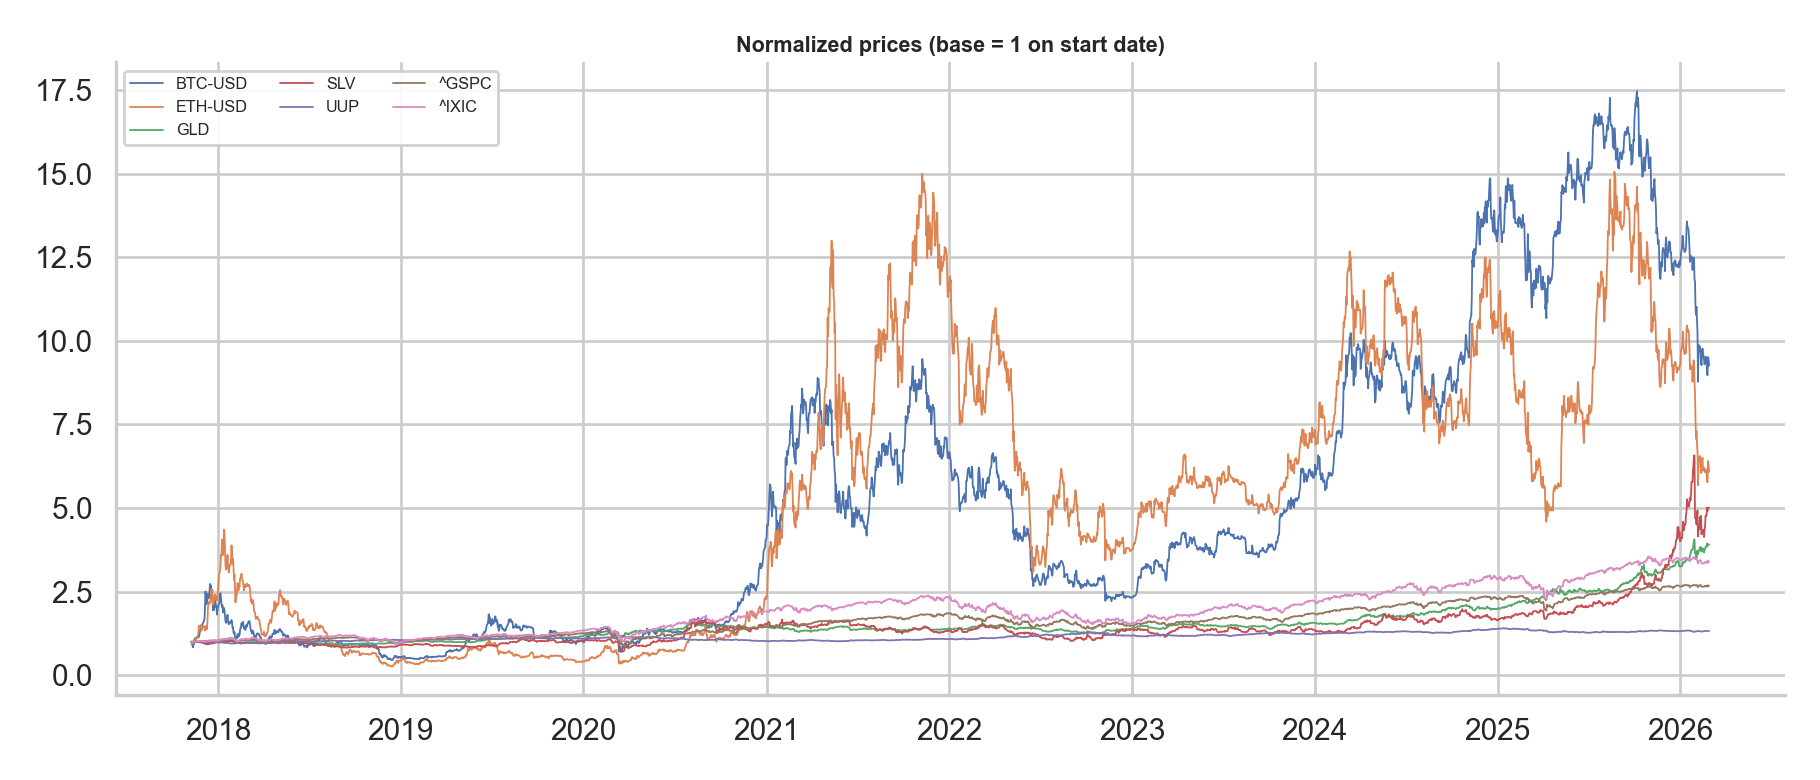
\includegraphics[width=0.95\textwidth]{../outputs/figures/eda_normalized_prices.png}
    \caption{Normalized prices of the assets included in the study.}
    \label{fig:eda_prices_appendix}
\end{figure}

Figure~\ref{fig:eda_vol_appendix} shows rolling volatility profiles. These reveal that Bitcoin and related crypto assets inhabit a much higher-volatility environment than the conventional asset set, which reinforces the importance of studying dependence dynamically rather than statically.

\begin{figure}[H]
    \centering
    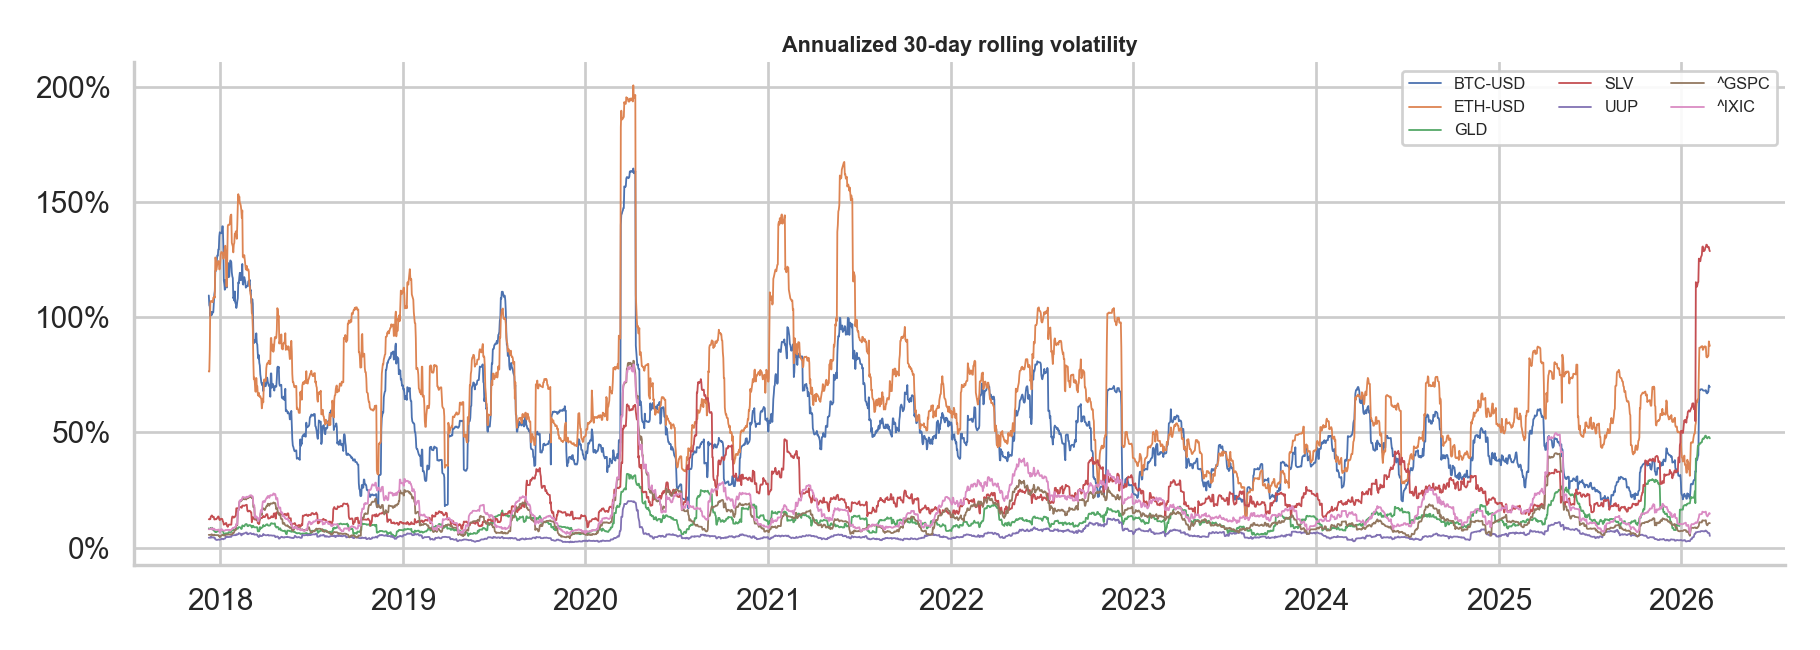
\includegraphics[width=0.95\textwidth]{../outputs/figures/eda_rolling_vol.png}
    \caption{Rolling volatility across the asset universe.}
    \label{fig:eda_vol_appendix}
\end{figure}

Figure~\ref{fig:eda_heatmap_appendix} provides the static correlation heatmap, while Figure~\ref{fig:eda_rollcorr_appendix} illustrates the dynamic rolling-correlation structure. Together, they motivate the main modeling choice of the thesis: static summaries are insufficient for describing the cross-market relations under study.

\begin{figure}[H]
    \centering
    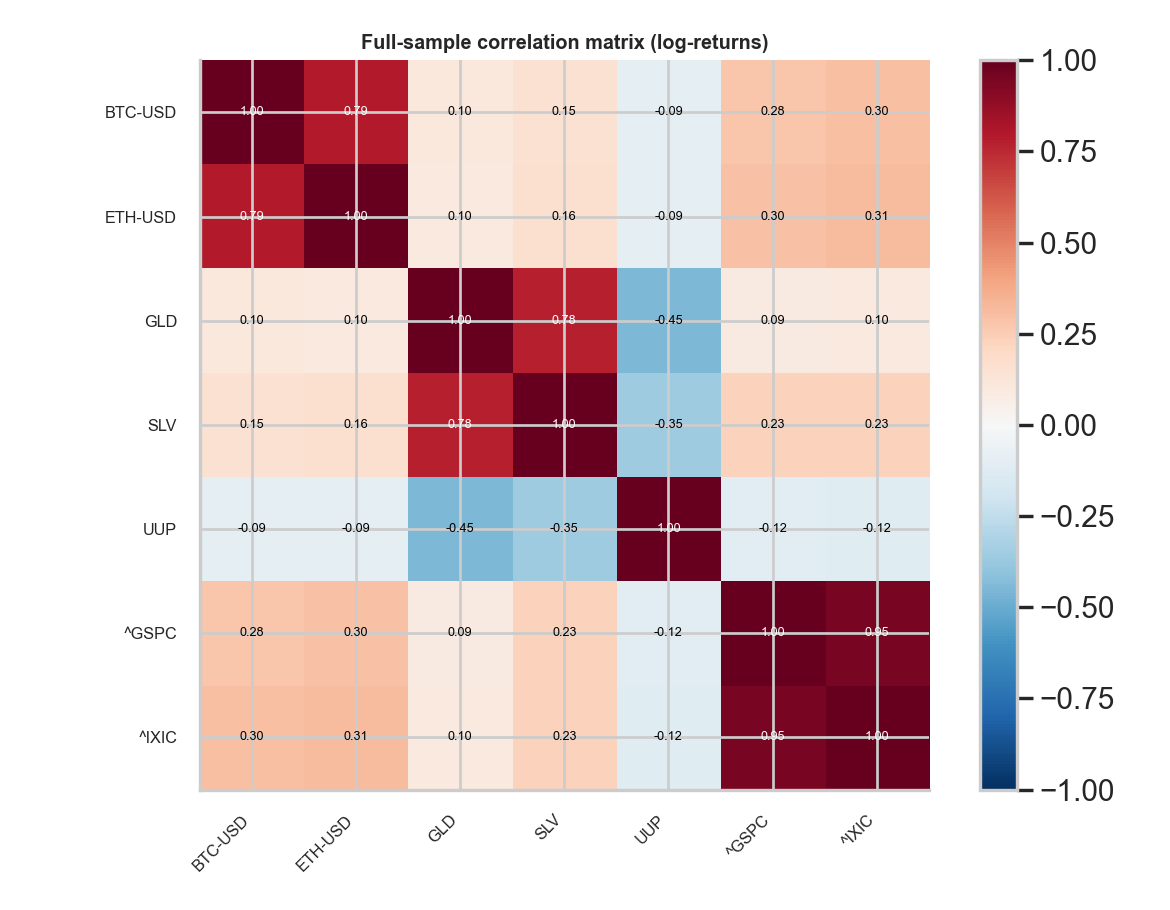
\includegraphics[width=0.85\textwidth]{../outputs/figures/eda_corr_heatmap.png}
    \caption{Static correlation heatmap of the return series.}
    \label{fig:eda_heatmap_appendix}
\end{figure}

\begin{figure}[H]
    \centering
    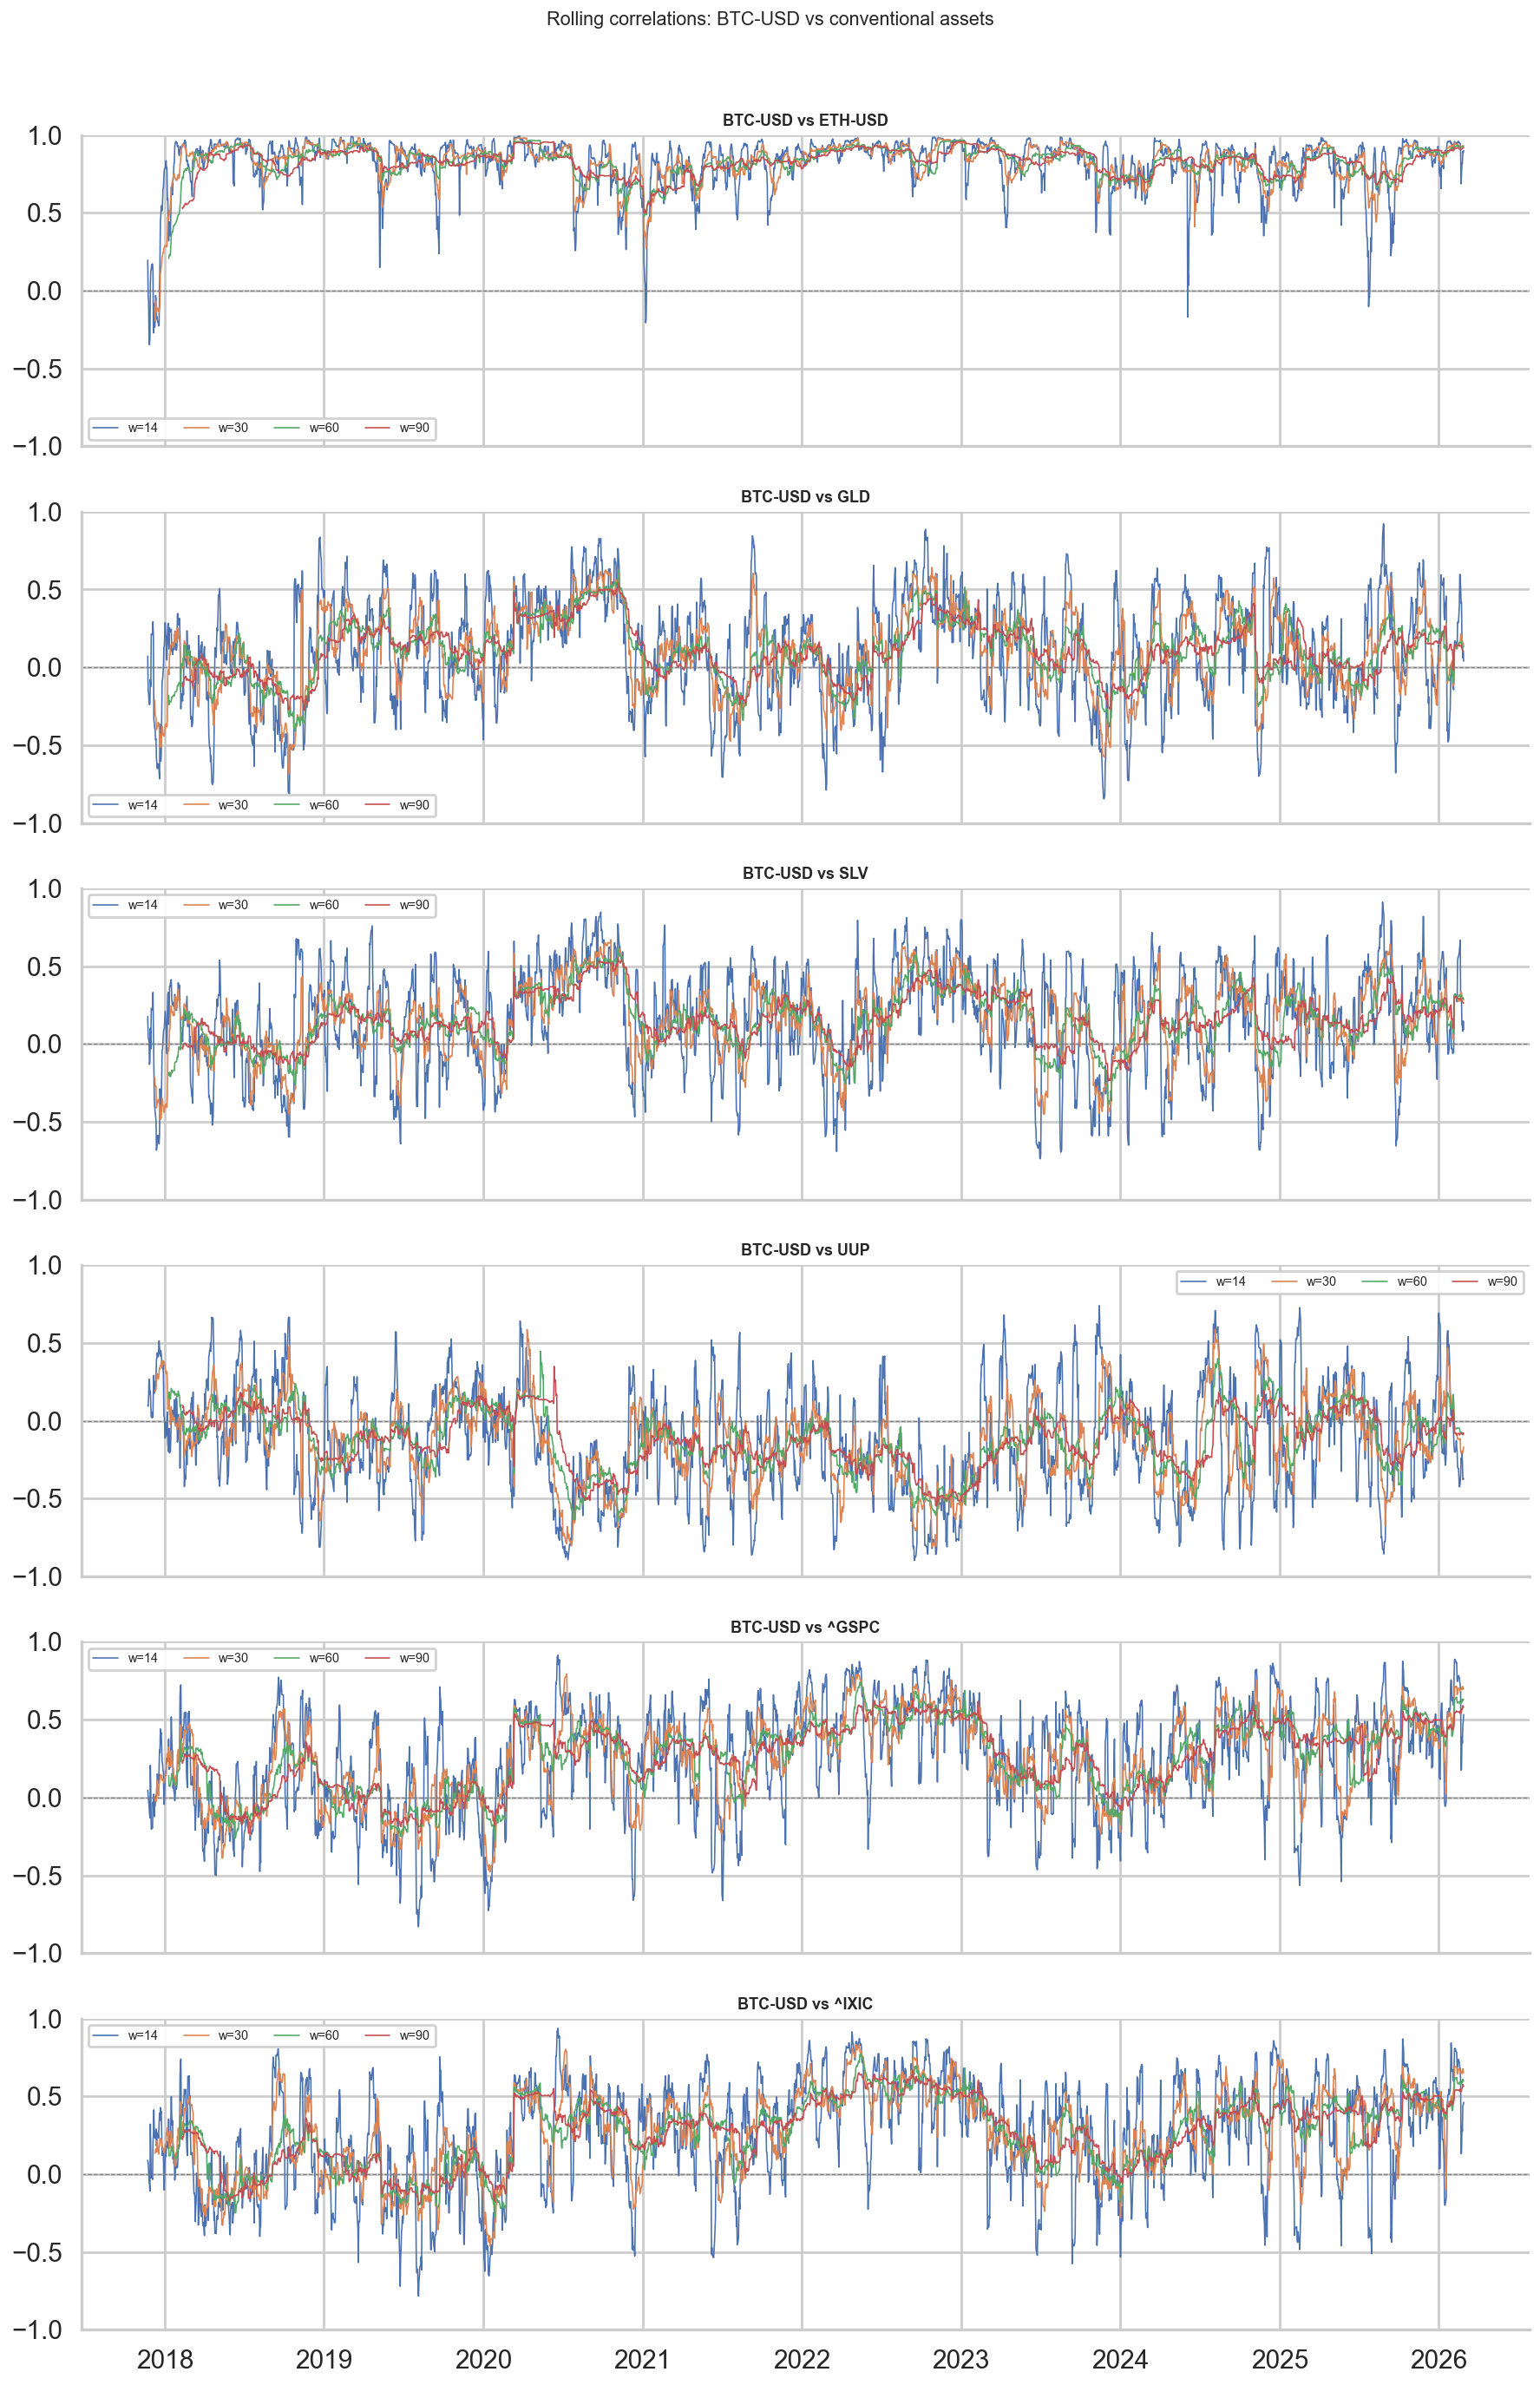
\includegraphics[width=0.98\textwidth]{../outputs/figures/eda_rolling_corr_all.png}
    \caption{Rolling correlation overview for the asset universe.}
    \label{fig:eda_rollcorr_appendix}
\end{figure}

\subsection{Why multiple rolling windows are used}

The thesis uses 14-day, 30-day, 60-day, and 90-day windows because no single dependence horizon is universally appropriate. A short window is more sensitive to recent shocks, but also noisier. A longer window produces a smoother target and often stronger persistence, but may react slowly to a regime shift. Evaluating several windows allows the empirical analysis to separate these effects.

The results indicate that the choice of window strongly shapes the forecastability profile. Longer windows are generally easier to forecast because they are smoother, but their predictive success is also more persistence-driven. Shorter windows react more quickly and are therefore more informative about local instability, although at the cost of noisier target behavior.

\subsection{Additional implementation remarks}

The project is organized so that each run of the pipeline produces consistent outputs in the \texttt{outputs/results}, \texttt{outputs/tables}, \texttt{outputs/figures}, and \texttt{outputs/predictions} directories. This structure is helpful not only for reproducibility but also for writing. Since the tables and figures are generated directly from the code pipeline, the gap between experiment execution and thesis writing is reduced.

Another useful implementation detail is that the notebook environment was aligned with the pipeline. Readability improvements were introduced in the notebooks so that figures are interpretable, benchmarks are selected robustly, and helper functions can be reused without fragile path assumptions. This matters because, in practice, exploratory notebooks often become a weak point in academic projects if they drift away from the main pipeline.

\subsection{Summary}

The appendix confirms an important methodological point: the empirical environment studied in this thesis is heterogeneous, nonstationary in economic interpretation, and rich enough to justify a time-varying dependency framework. The descriptive evidence supports the modeling strategy used in the main body of the thesis.

\section{Appendix B: Supplementary Forecasting Results}

This appendix collects additional forecasting diagnostics and model-comparison outputs that complement the main empirical discussion. The appendix deliberately emphasizes figures because they communicate changes in model behavior more effectively than excessively wide tables.

\subsection{Model-comparison figures}

\begin{figure}[H]
    \centering
    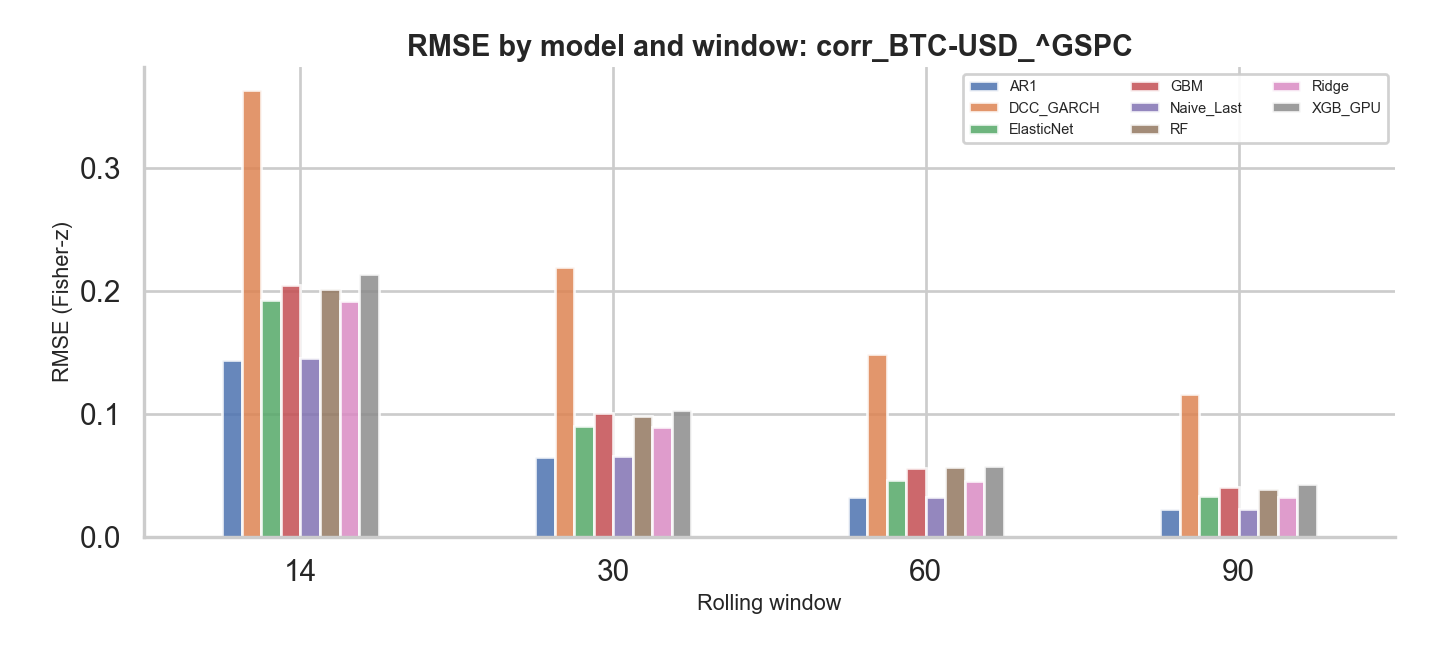
\includegraphics[width=0.8\textwidth]{../outputs/figures/model_rmse_comparison.png}
    \caption{Average RMSE comparison across model families.}
\end{figure}

\begin{figure}[H]
    \centering
    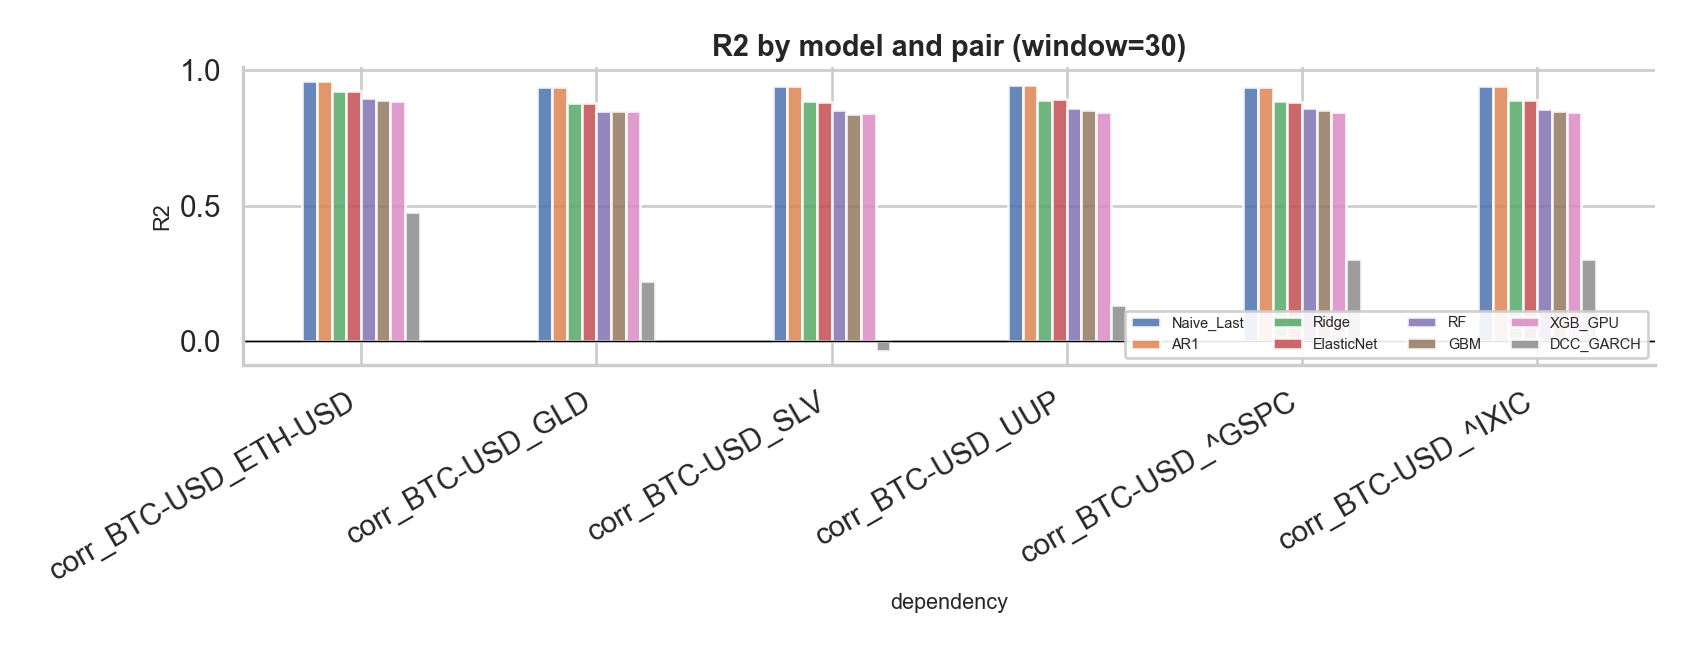
\includegraphics[width=0.8\textwidth]{../outputs/figures/model_r2_comparison_w30.png}
    \caption{Model $R^2$ comparison for the 30-day window.}
\end{figure}

\begin{figure}[H]
    \centering
    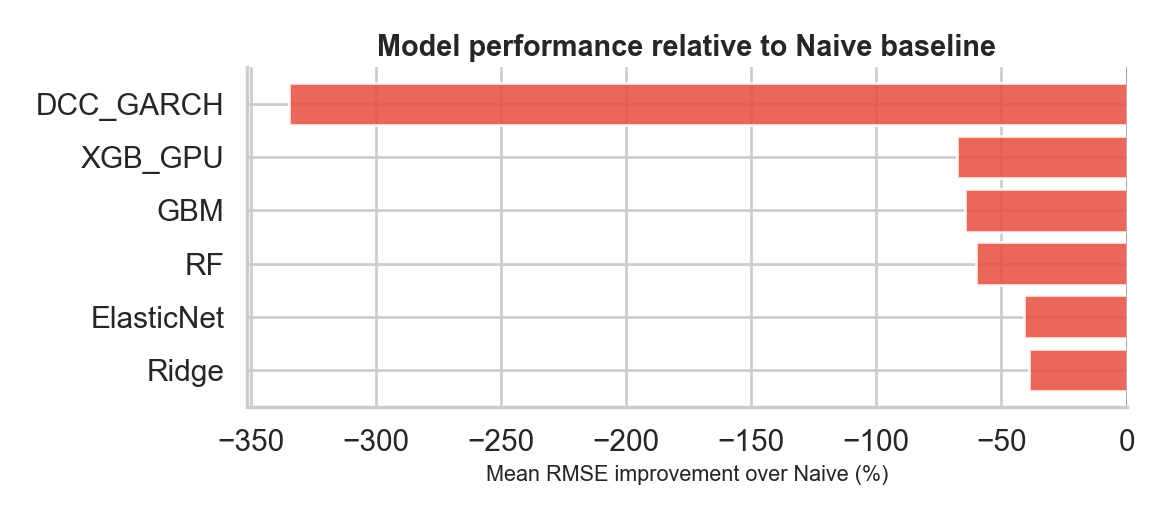
\includegraphics[width=0.8\textwidth]{../outputs/figures/model_improvement_over_naive.png}
    \caption{Improvement relative to the naive baseline.}
\end{figure}

\subsection{Hyperparameter and feature diagnostics}

\begin{figure}[H]
    \centering
    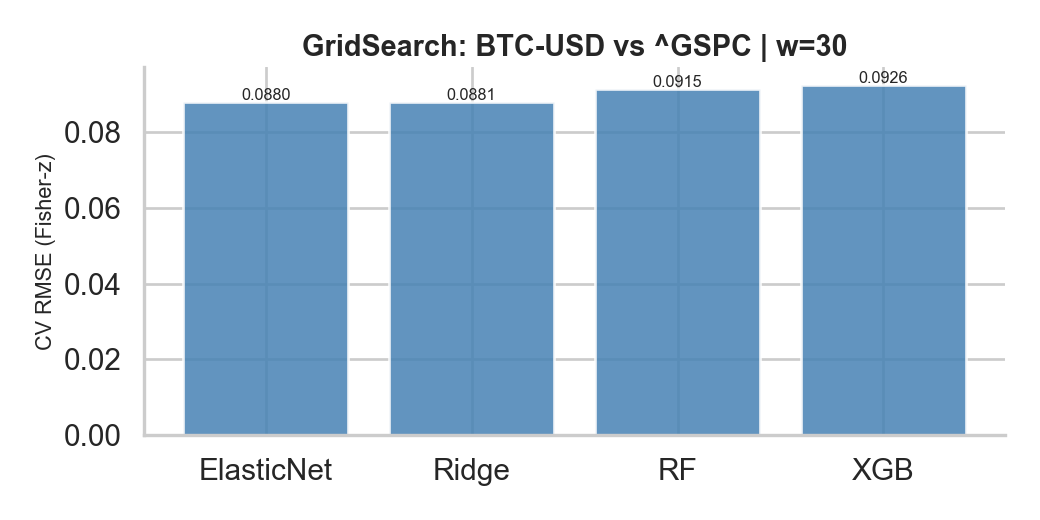
\includegraphics[width=0.8\textwidth]{../outputs/figures/gridsearch_cv_rmse_BTC-USD_^GSPC_w30.png}
    \caption{Grid-search cross-validation RMSE for the representative Bitcoin--S\&P 500 forecasting task.}
\end{figure}

\begin{figure}[H]
    \centering
    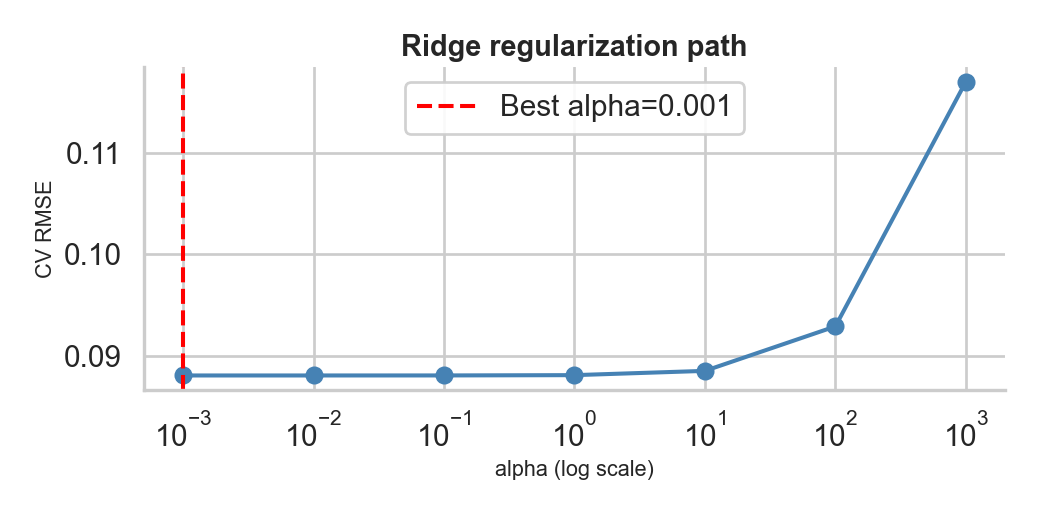
\includegraphics[width=0.8\textwidth]{../outputs/figures/ridge_regularization_path.png}
    \caption{Regularization path for the Ridge-based forecasting specification.}
\end{figure}

\begin{figure}[H]
    \centering
    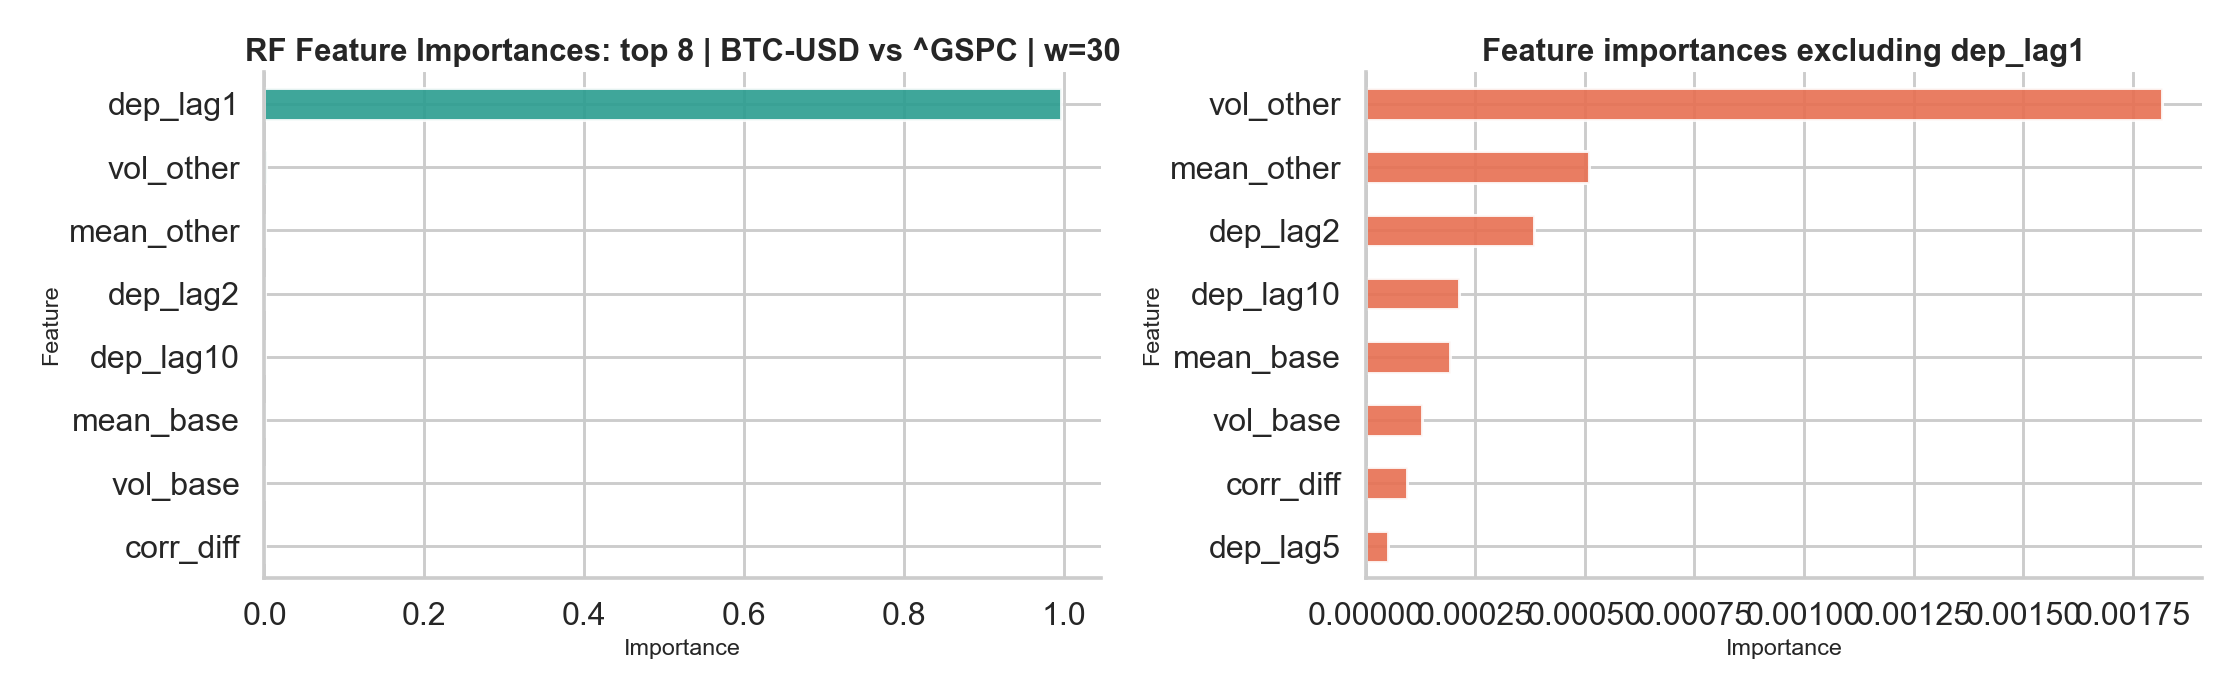
\includegraphics[width=0.85\textwidth]{../outputs/figures/rf_feature_importance_BTC-USD_^GSPC_w30_readable.png}
    \caption{Readable feature-importance view for the Random Forest model.}
\end{figure}

\subsection{Diagnostic plots for the representative equity pair}

\begin{figure}[H]
    \centering
    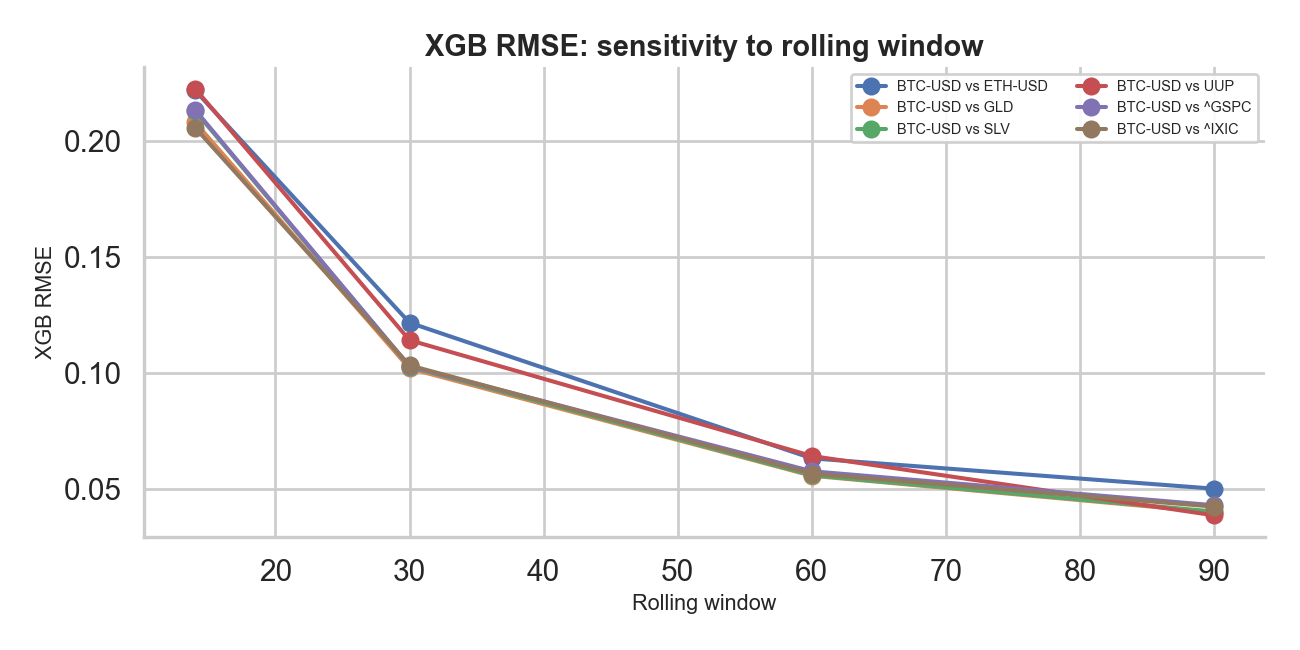
\includegraphics[width=0.82\textwidth]{../outputs/figures/xgb_window_sensitivity.png}
    \caption{Window sensitivity of the XGBoost-based forecasting layer.}
\end{figure}

\begin{figure}[H]
    \centering
    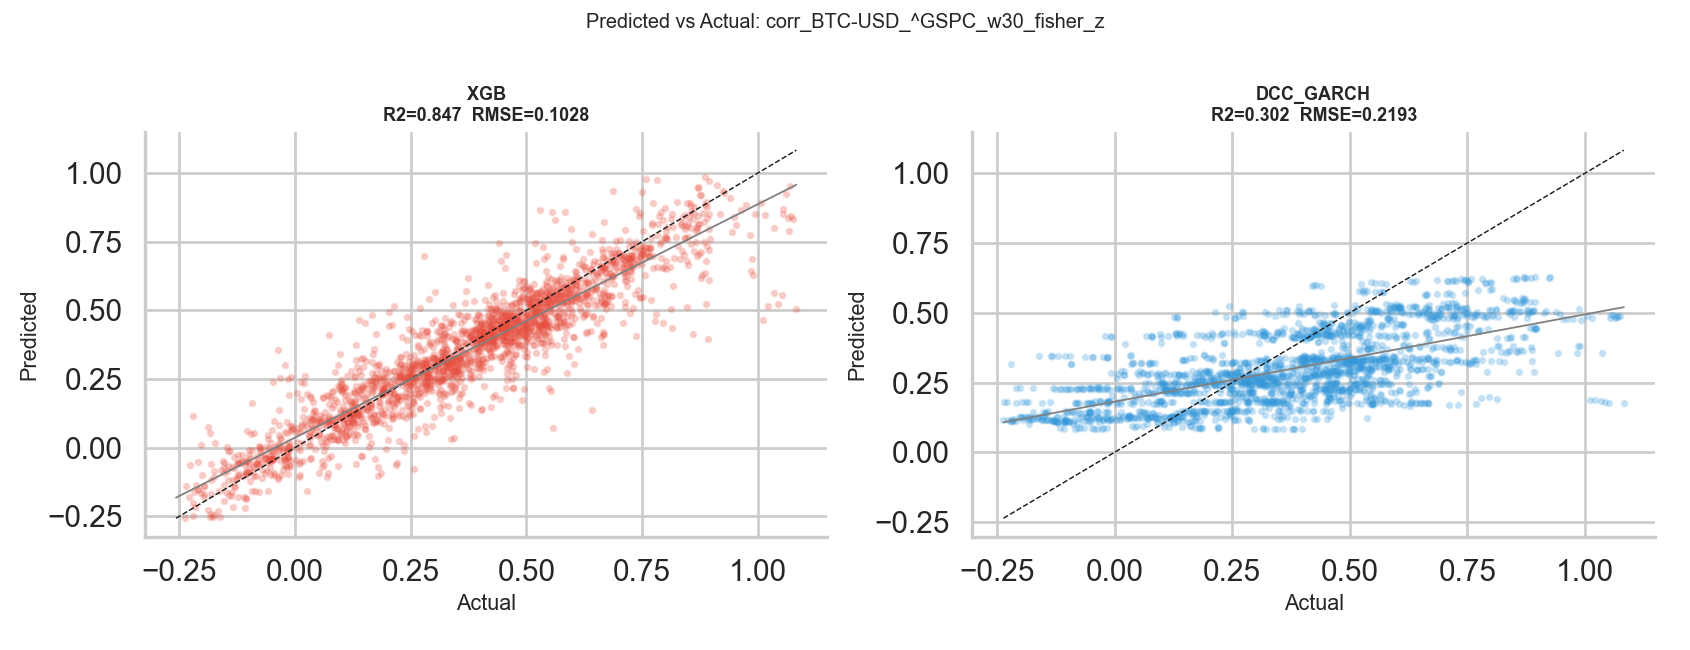
\includegraphics[width=0.82\textwidth]{../outputs/figures/scatter_corr_BTC-USD_^GSPC_w30_fisher_z.png}
    \caption{Forecast scatter diagnostic for the Bitcoin--S\&P 500 dependency experiment.}
\end{figure}

\begin{figure}[H]
    \centering
    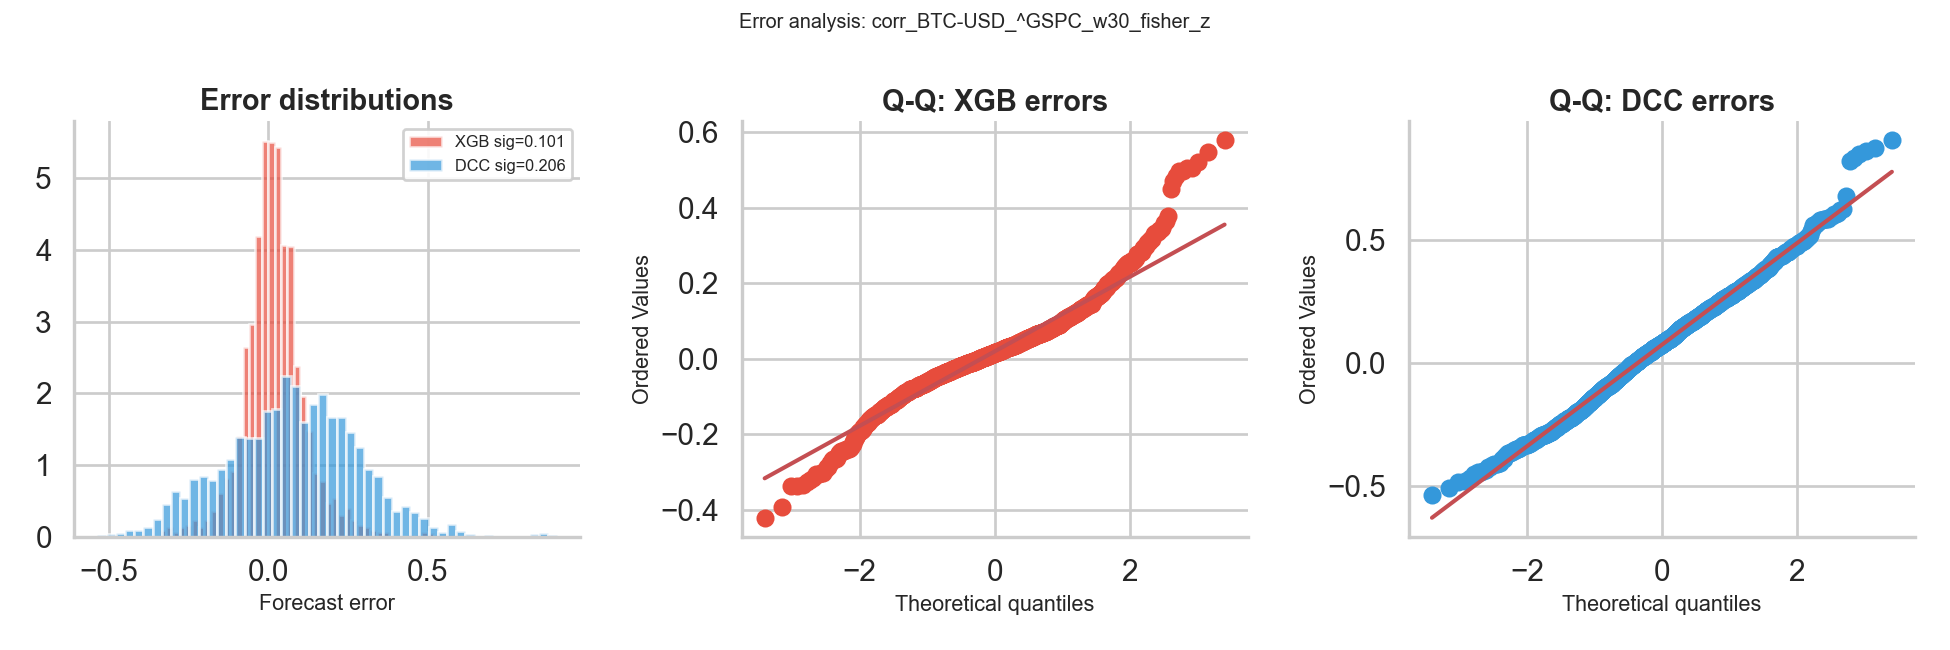
\includegraphics[width=0.82\textwidth]{../outputs/figures/error_dist_corr_BTC-USD_^GSPC_w30_fisher_z.png}
    \caption{Forecast error distribution for the representative Bitcoin--S\&P 500 dependency experiment.}
\end{figure}

\subsection{Sensitivity by asset pair}

\begin{figure}[H]
    \centering
    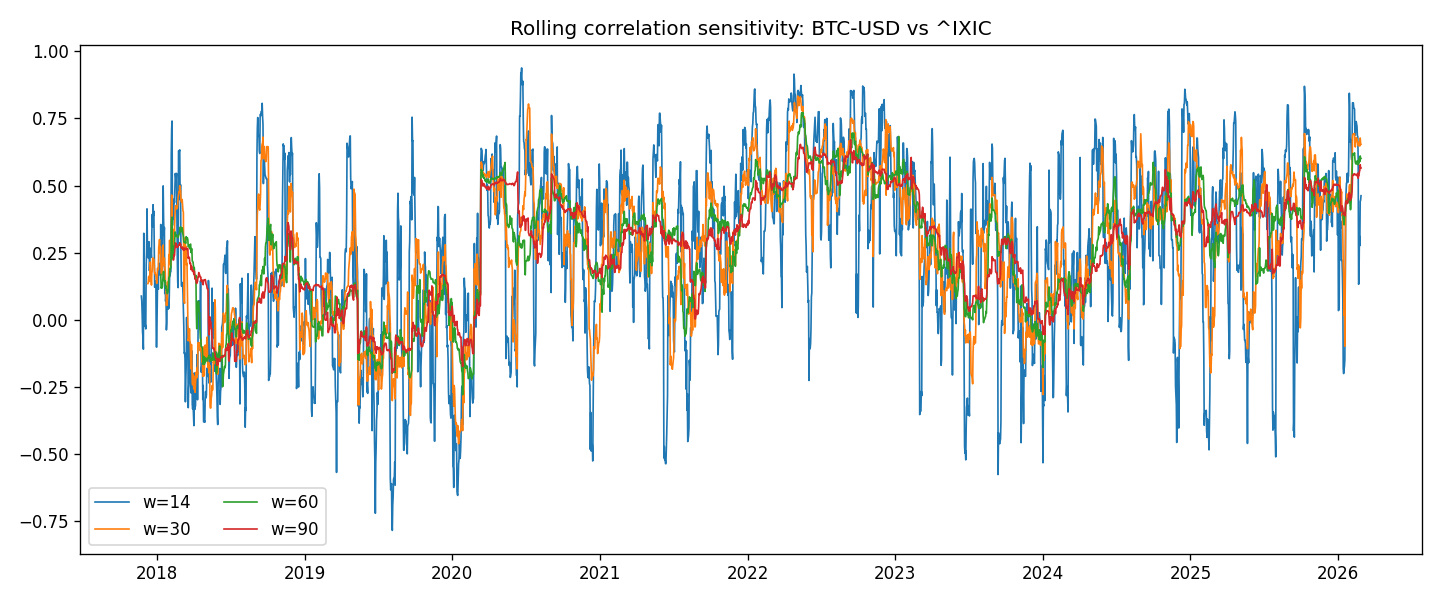
\includegraphics[width=0.9\textwidth]{../outputs/figures/sensitivity_BTC-USD_^IXIC.png}
    \caption{Sensitivity analysis for the Bitcoin--NASDAQ pair.}
\end{figure}

\begin{figure}[H]
    \centering
    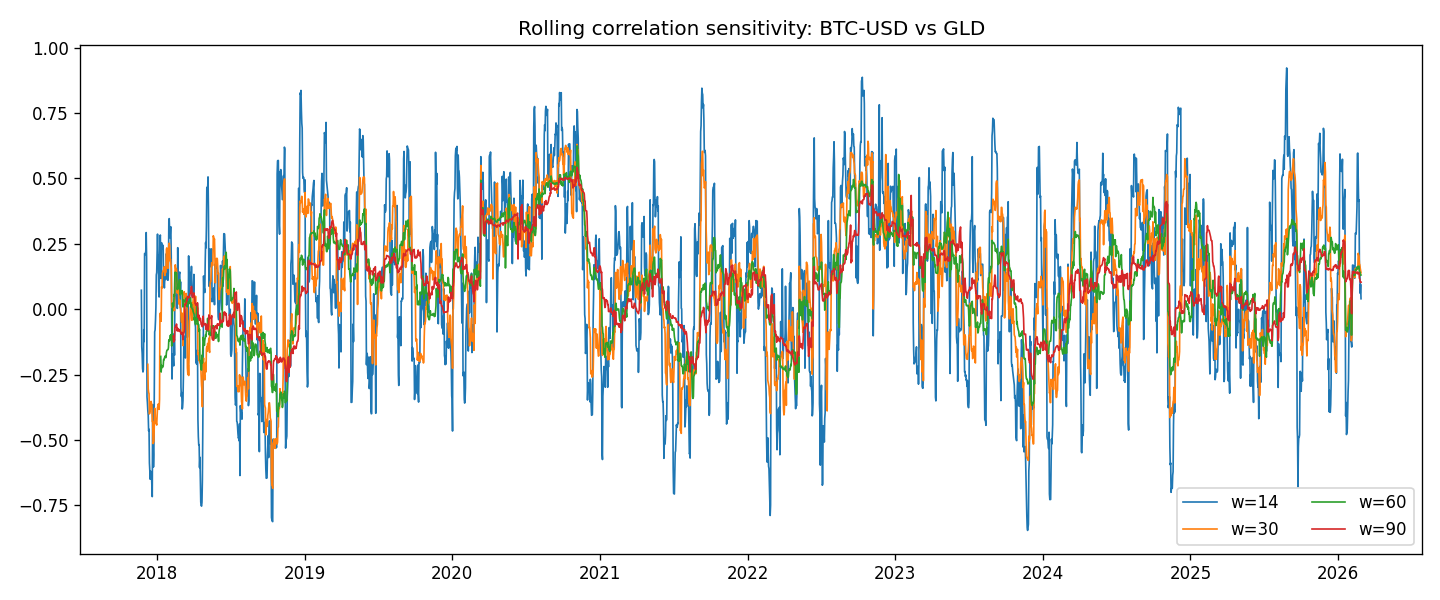
\includegraphics[width=0.9\textwidth]{../outputs/figures/sensitivity_BTC-USD_GLD.png}
    \caption{Sensitivity analysis for the Bitcoin--gold pair.}
\end{figure}

\begin{figure}[H]
    \centering
    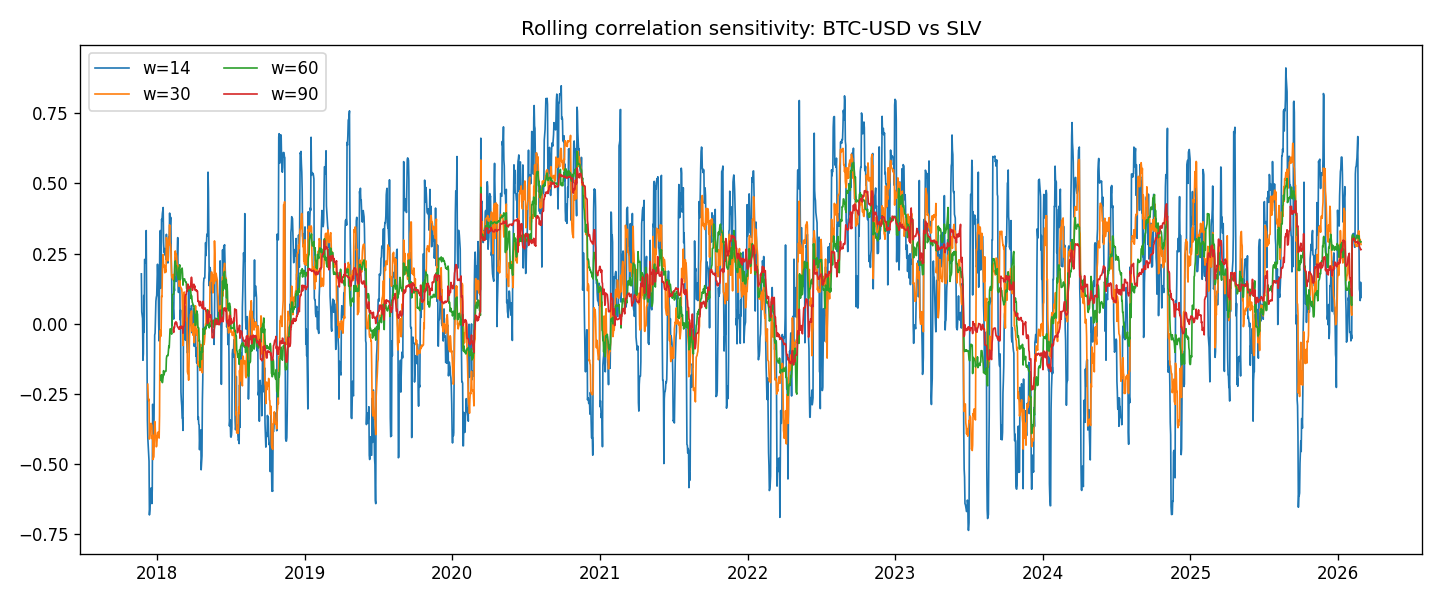
\includegraphics[width=0.9\textwidth]{../outputs/figures/sensitivity_BTC-USD_SLV.png}
    \caption{Sensitivity analysis for the Bitcoin--silver pair.}
\end{figure}

\begin{figure}[H]
    \centering
    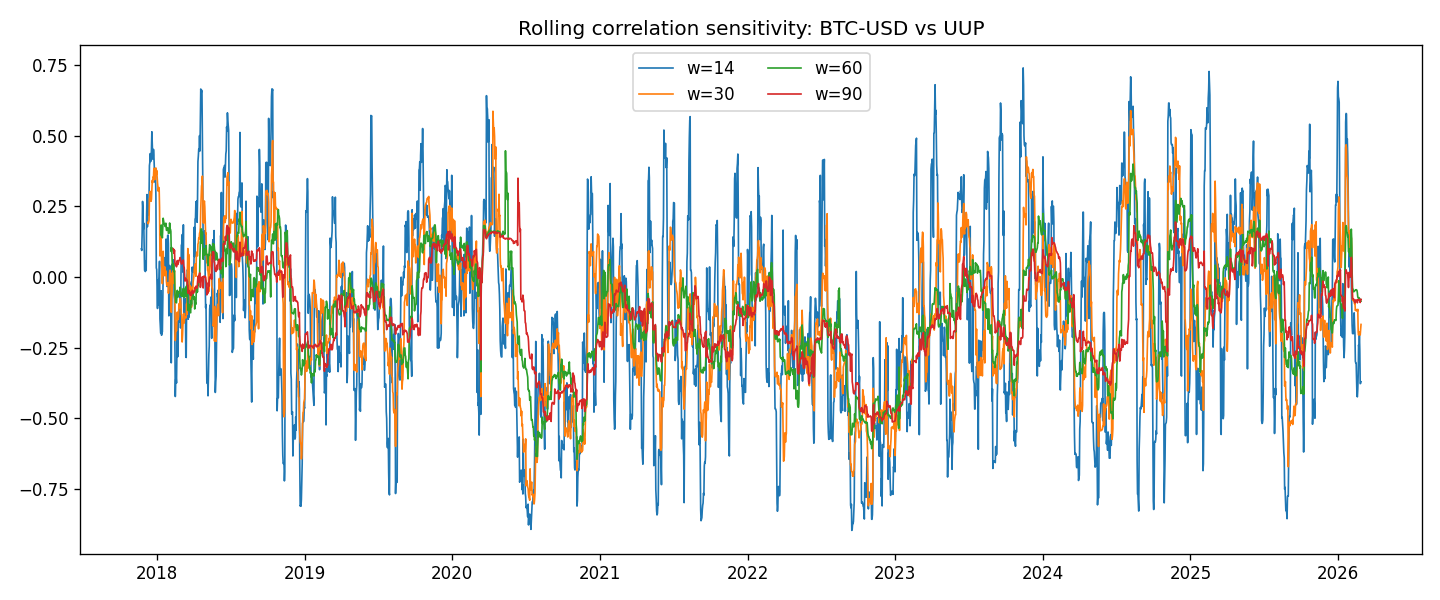
\includegraphics[width=0.9\textwidth]{../outputs/figures/sensitivity_BTC-USD_UUP.png}
    \caption{Sensitivity analysis for the Bitcoin--UUP pair.}
\end{figure}

\begin{figure}[H]
    \centering
    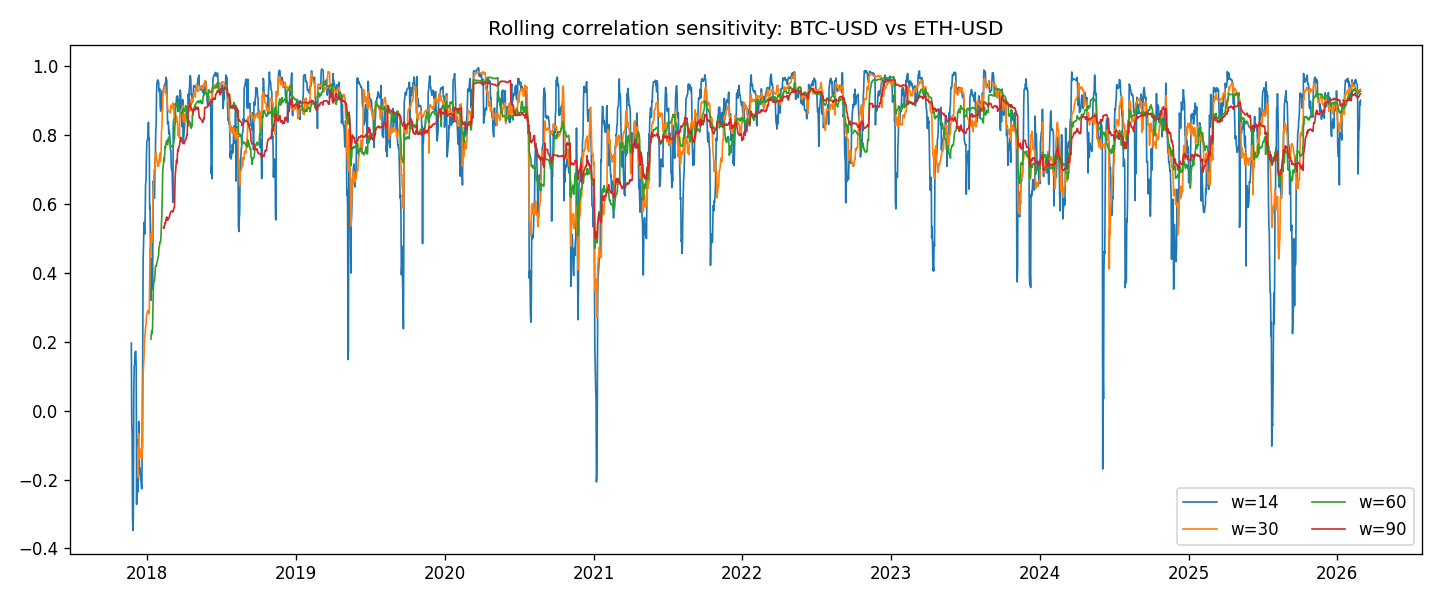
\includegraphics[width=0.9\textwidth]{../outputs/figures/sensitivity_BTC-USD_ETH-USD.png}
    \caption{Sensitivity analysis for the Bitcoin--Ethereum pair.}
\end{figure}

\subsection{Interpretation}

The supplementary figures reinforce several points made in the main text. Forecast quality depends materially on the choice of rolling window, the target remains strongly persistence-driven, and performance differences across model families are easier to interpret through comparative visuals than through a single ranking statistic alone.

\section{Appendix C: Supplementary Signal-Layer Results}

This appendix presents additional material for the investor-oriented warning layer.

\subsection{Signal figures by asset}

\begin{figure}[H]
    \centering
    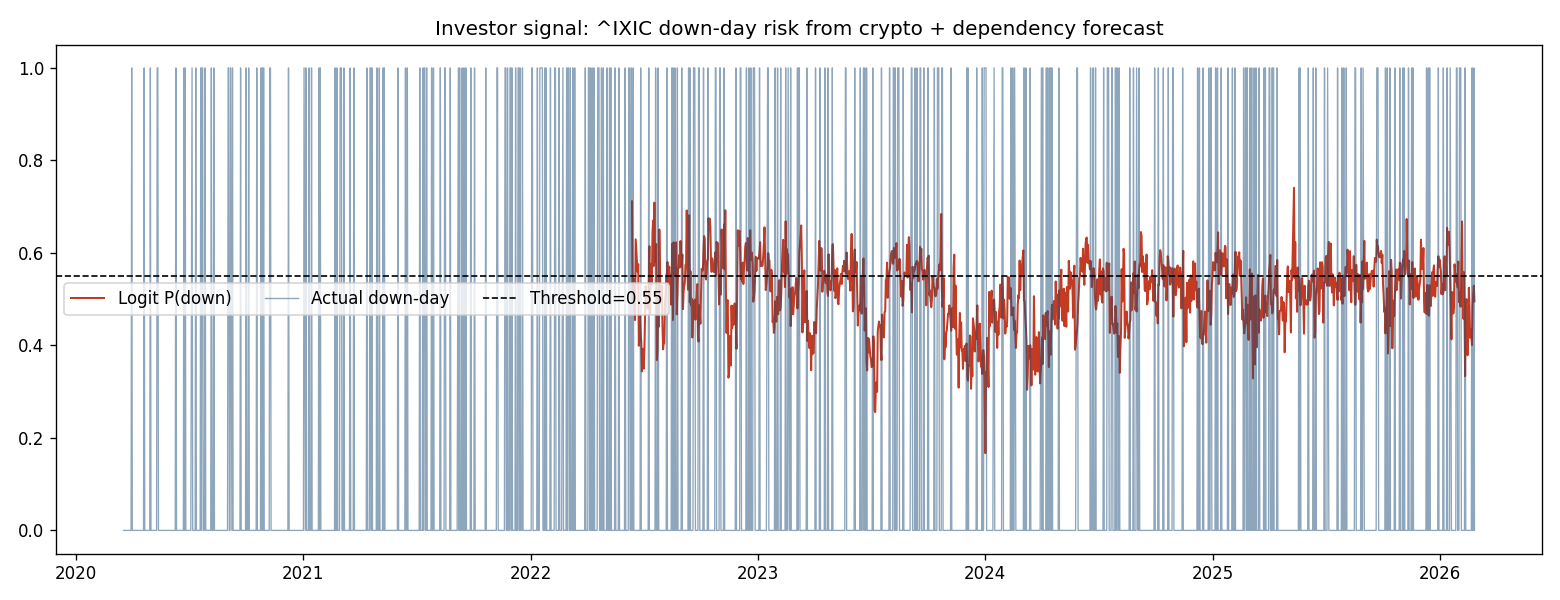
\includegraphics[width=0.9\textwidth]{../outputs/figures/signal_corr_BTC-USD_^IXIC_w30.png}
    \caption{Signal-layer output for the Bitcoin--NASDAQ relation at the 30-day window.}
\end{figure}

\begin{figure}[H]
    \centering
    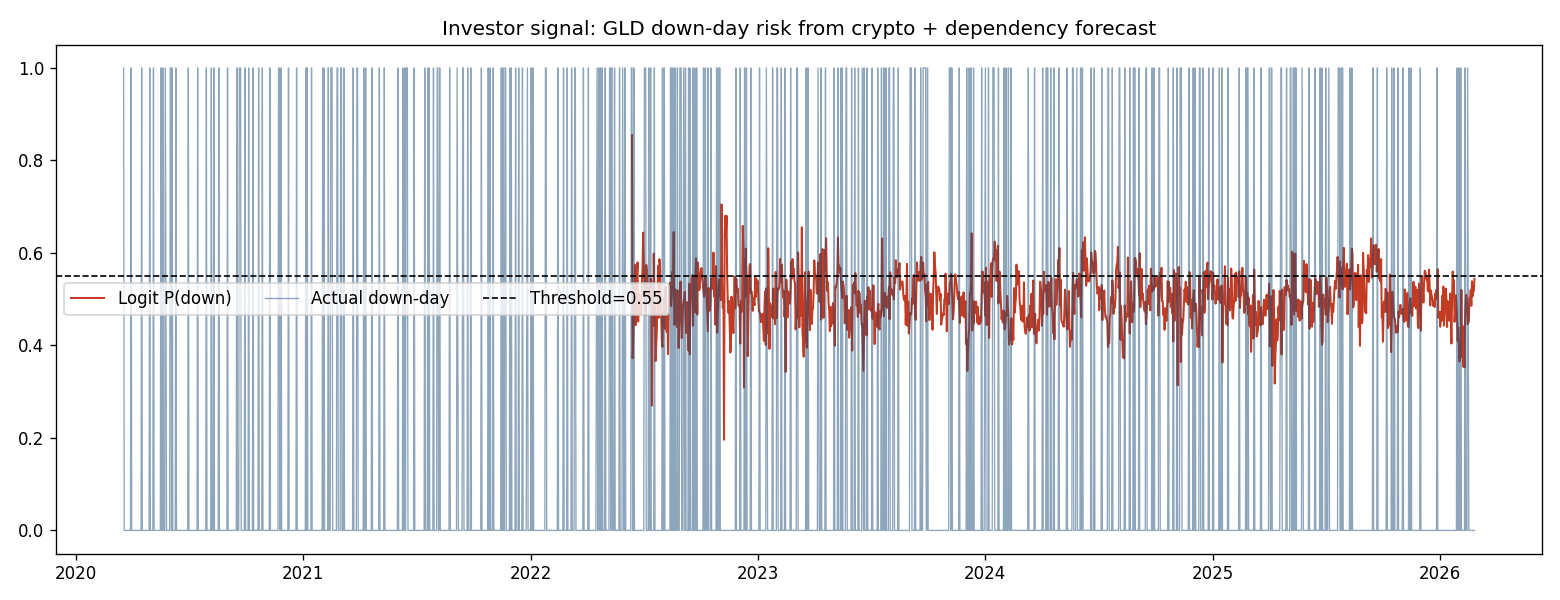
\includegraphics[width=0.9\textwidth]{../outputs/figures/signal_corr_BTC-USD_GLD_w30.png}
    \caption{Signal-layer output for the Bitcoin--gold relation at the 30-day window.}
\end{figure}

\begin{figure}[H]
    \centering
    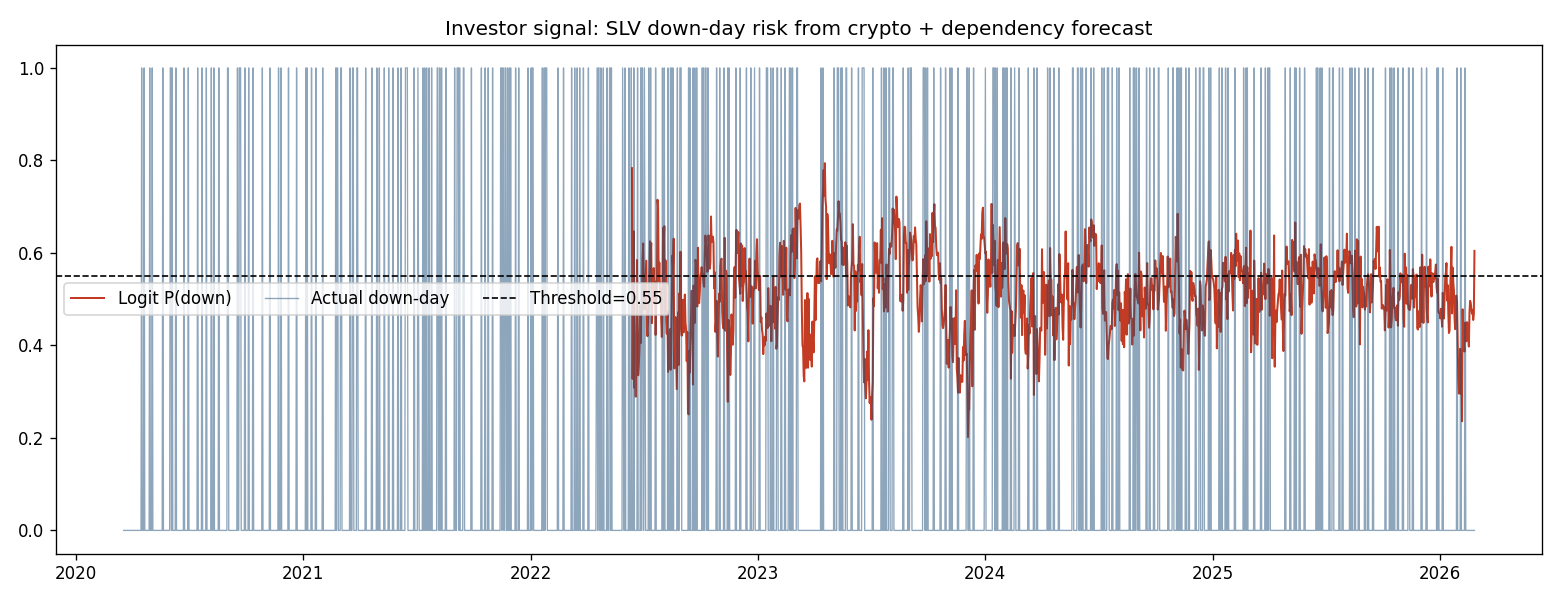
\includegraphics[width=0.9\textwidth]{../outputs/figures/signal_corr_BTC-USD_SLV_w30.png}
    \caption{Signal-layer output for the Bitcoin--silver relation at the 30-day window.}
\end{figure}

\begin{figure}[H]
    \centering
    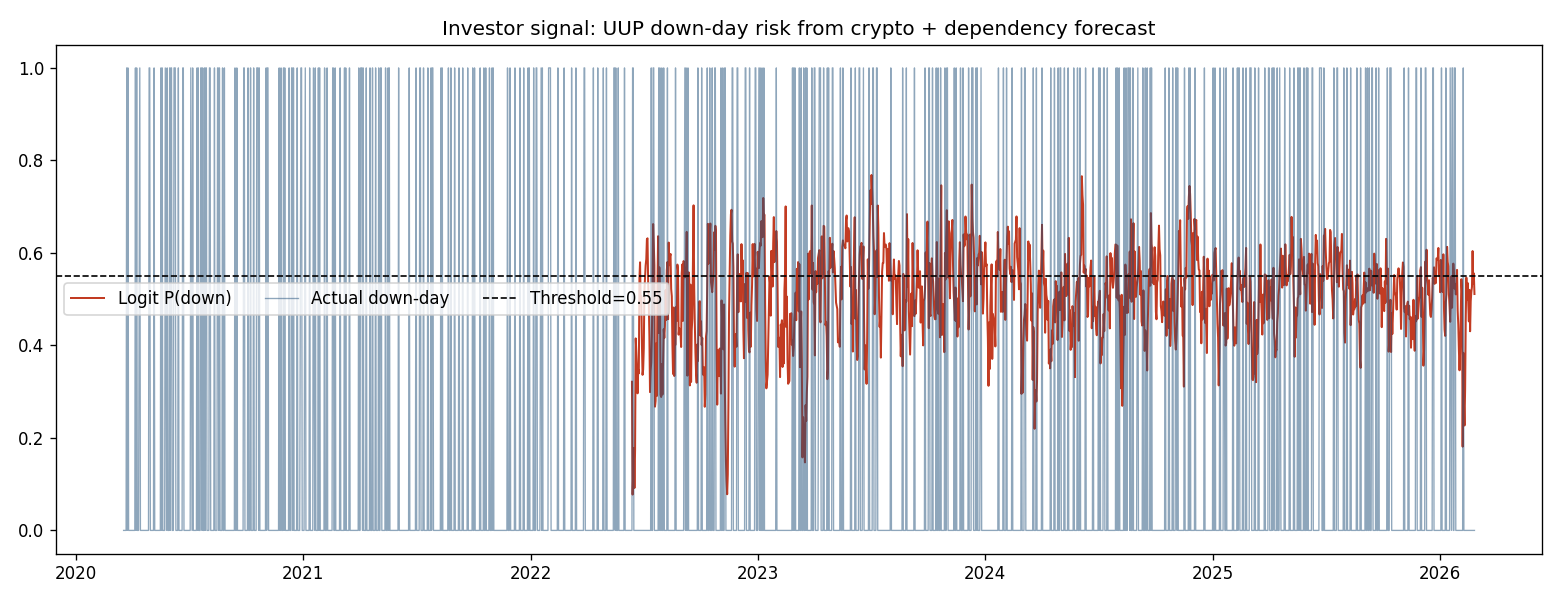
\includegraphics[width=0.9\textwidth]{../outputs/figures/signal_corr_BTC-USD_UUP_w30.png}
    \caption{Signal-layer output for the Bitcoin--UUP relation at the 30-day window.}
\end{figure}

\subsection{Cross-market warning interpretation}

The supplementary signal figures show that the practical layer behaves differently across markets. Equity-related targets display somewhat clearer warning episodes, while the metal and dollar-linked targets are noisier and weaker. This asymmetry is economically sensible and supports the interpretation that the investor layer should be used selectively rather than uniformly.

\subsection{Summary table}

\begin{table}[H]
    \centering
    \caption{Average signal-layer performance by classifier family.}
    \begin{tabular}{lrrr}
        \toprule
        Signal model & Balanced Accuracy & F1\_down & AUC \\
        \midrule
        Logit & 0.506 & 0.209 & 0.508 \\
        GBM\_Cls & 0.501 & 0.033 & 0.520 \\
        RF\_Cls & 0.500 & 0.030 & 0.519 \\
        \bottomrule
    \end{tabular}
\end{table}

These summary values confirm that the signal layer is meaningful but modest. Its strongest role is as a supplementary warning mechanism rather than as a standalone allocator.

\clearpage
\begin{figure}[p]
    \centering
    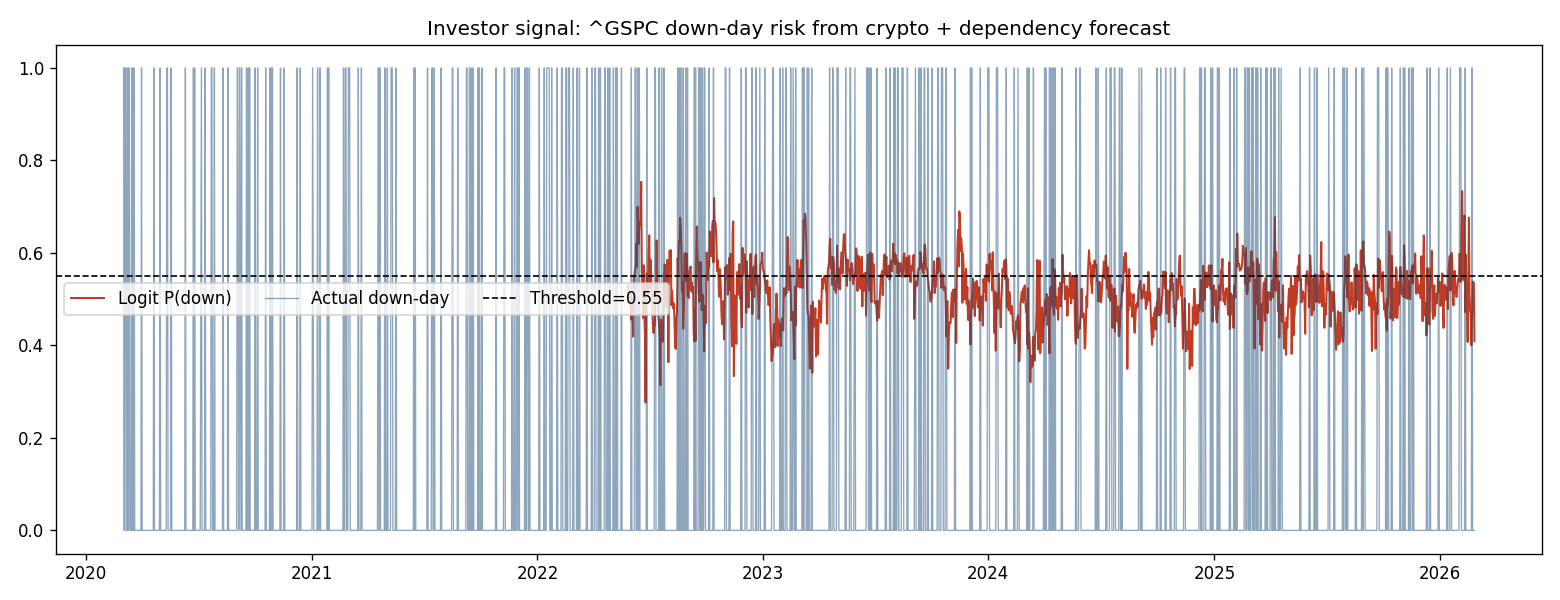
\includegraphics[width=0.95\textwidth]{../outputs/figures/signal_corr_BTC-USD_^GSPC_w14.png}
    \caption{Supplementary S\&P 500 warning signal at the 14-day window.}
\end{figure}

\clearpage
\begin{figure}[p]
    \centering
    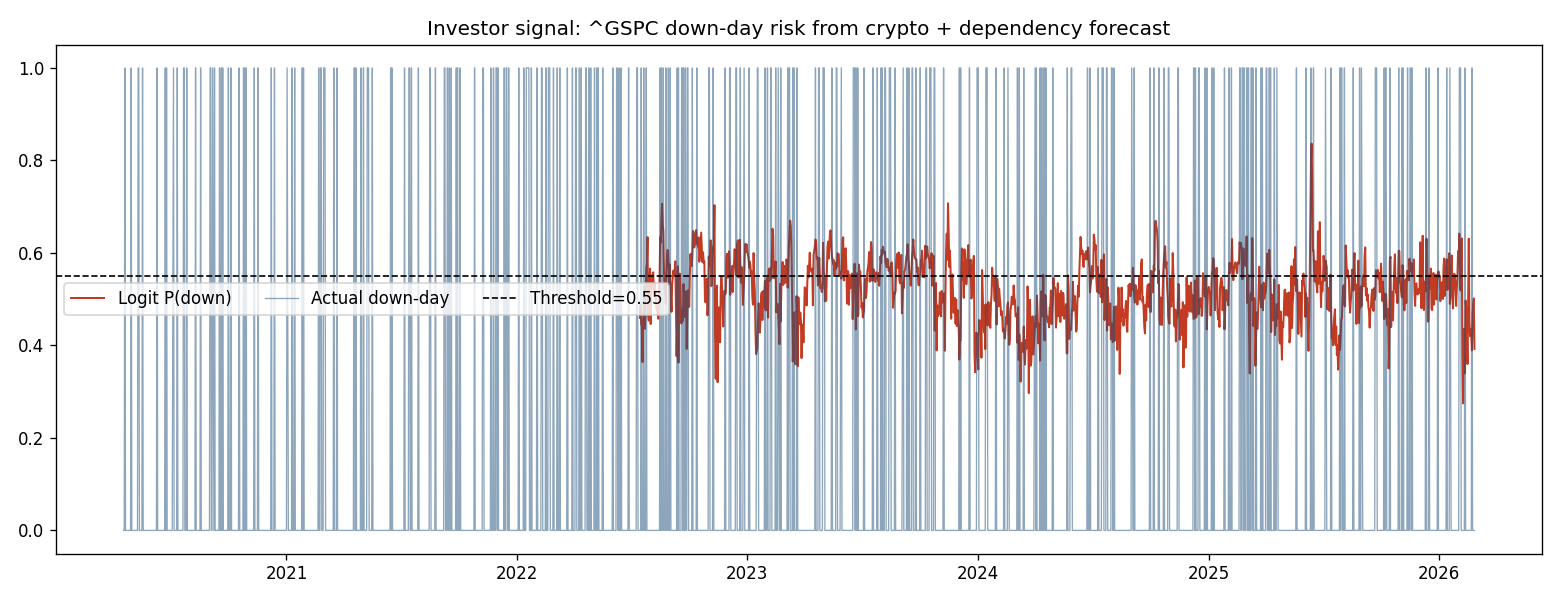
\includegraphics[width=0.95\textwidth]{../outputs/figures/signal_corr_BTC-USD_^GSPC_w60.png}
    \caption{Supplementary S\&P 500 warning signal at the 60-day window.}
\end{figure}

\clearpage
\begin{figure}[p]
    \centering
    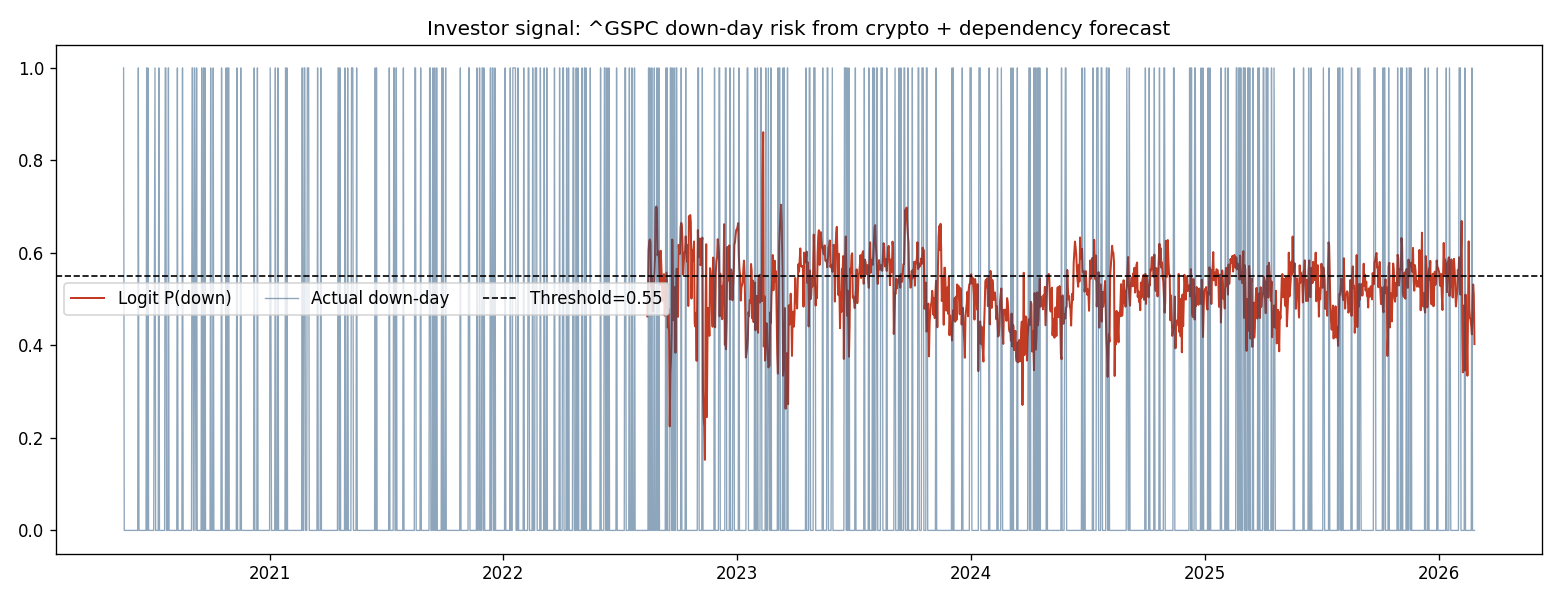
\includegraphics[width=0.95\textwidth]{../outputs/figures/signal_corr_BTC-USD_^GSPC_w90.png}
    \caption{Supplementary S\&P 500 warning signal at the 90-day window.}
\end{figure}

\clearpage
\begin{figure}[p]
    \centering
    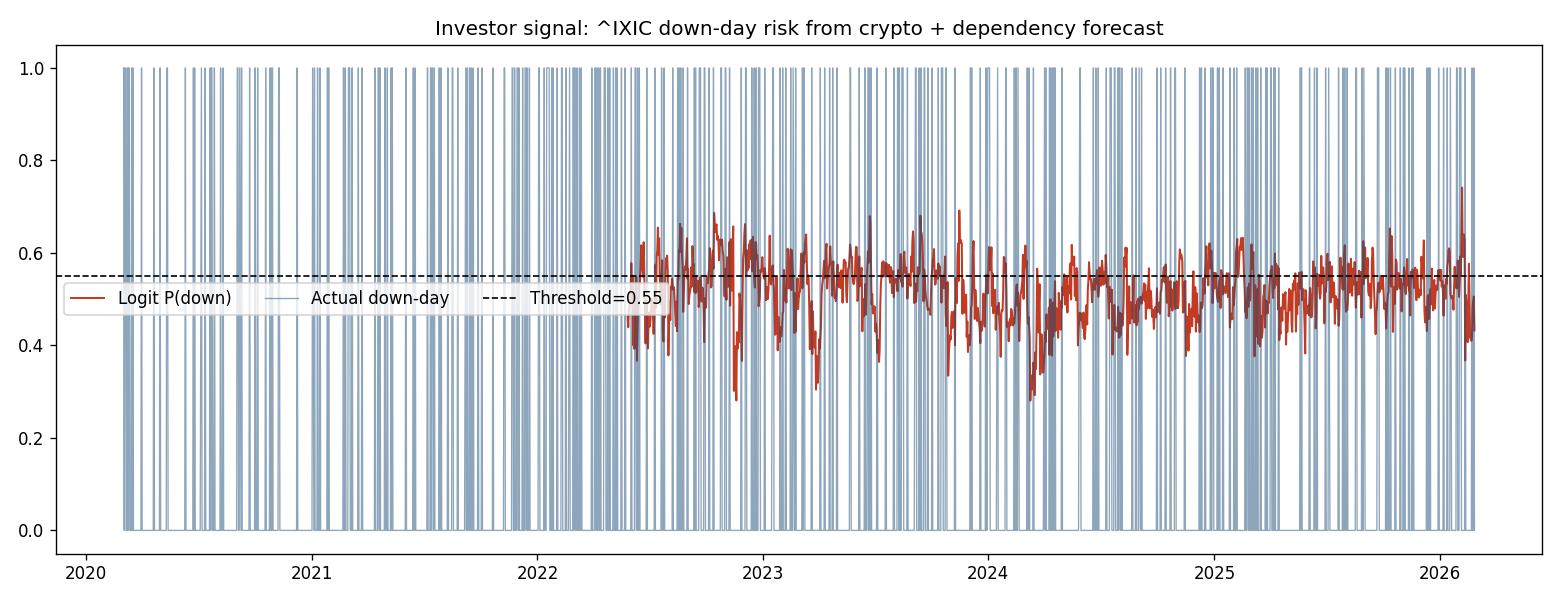
\includegraphics[width=0.95\textwidth]{../outputs/figures/signal_corr_BTC-USD_^IXIC_w14.png}
    \caption{Supplementary NASDAQ warning signal at the 14-day window.}
\end{figure}

\clearpage
\begin{figure}[p]
    \centering
    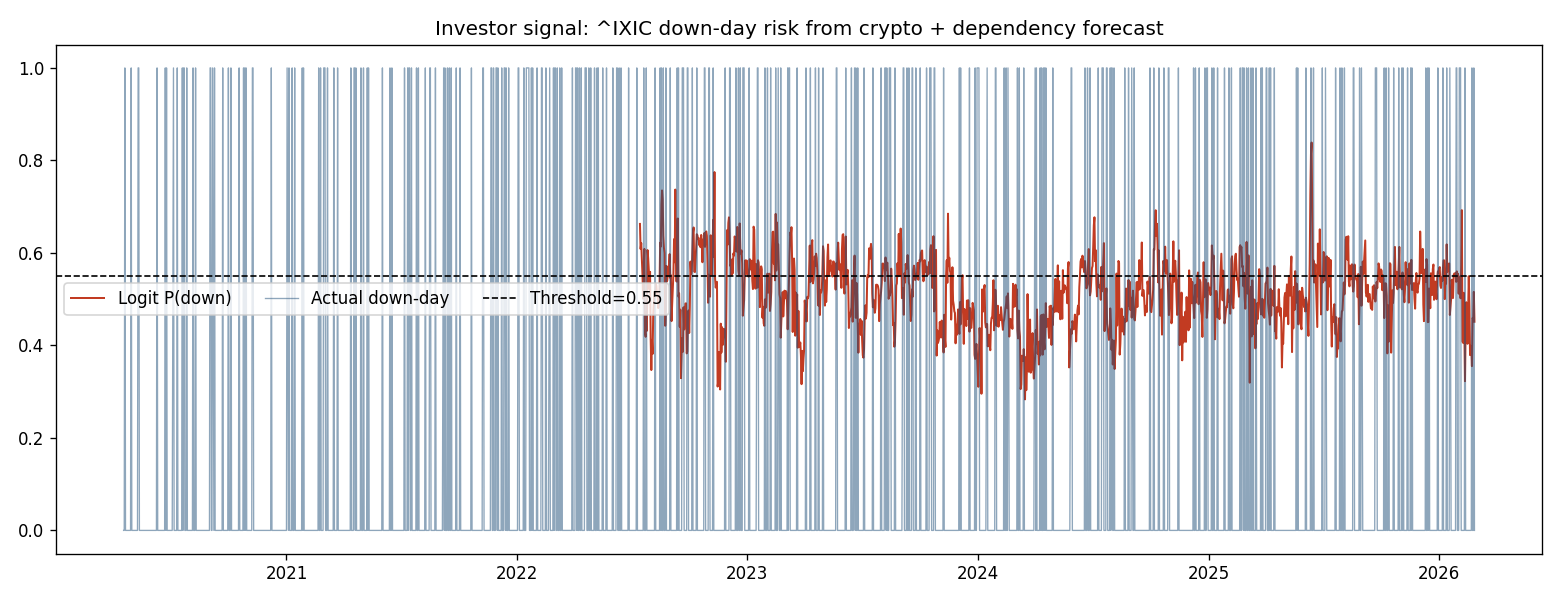
\includegraphics[width=0.95\textwidth]{../outputs/figures/signal_corr_BTC-USD_^IXIC_w60.png}
    \caption{Supplementary NASDAQ warning signal at the 60-day window.}
\end{figure}

\section{Appendix D: Reproducibility and Code Structure}

\subsection{Project organization}

The computational part of the thesis is structured as a reproducible research project rather than a collection of disconnected scripts. The main directories are organized as follows:

\begin{table}[H]
    \centering
    \caption{Simplified project structure.}
    \begin{tabular}{ll}
        \toprule
        Path & Role \\
        \midrule
        \texttt{thesis\_app/} & Core Python modules for the pipeline \\
        \texttt{notebooks/} & Exploratory and presentation-oriented notebooks \\
        \texttt{data/raw/} & Cached downloaded price data \\
        \texttt{data/processed/} & Derived returns and processed datasets \\
        \texttt{outputs/results/} & CSV summaries of experiments \\
        \texttt{outputs/tables/} & LaTeX-exported tables \\
        \texttt{outputs/figures/} & Forecast, EDA, and signal figures \\
        \texttt{thesis/} & Final thesis document and appendices \\
        \bottomrule
    \end{tabular}
\end{table}

\subsection{Main implementation modules}

The following modules constitute the core of the forecasting system:

\begin{itemize}
    \item \texttt{pipeline.py}: orchestrates the full dependency-forecasting and signal-generation workflow.
    \item \texttt{dcc\_walk.py}: contains the leakage-safe walk-forward DCC-GARCH implementation.
    \item \texttt{signal\_layer.py}: defines the investor warning layer and associated classification metrics.
    \item \texttt{notebook\_helpers.py}: provides consistent styling and helper routines for notebook-based analysis.
\end{itemize}

This separation of concerns is useful both scientifically and practically. Scientifically, it makes the logic of the workflow easier to audit. Practically, it allows individual modules to be tested or improved without rewriting the entire system.

\subsection{Execution flow}

At a high level, the execution flow can be summarized as follows:

\begin{enumerate}
    \item Load configuration and path settings.
    \item Load or refresh raw price data.
    \item Compute synchronized log returns.
    \item Generate rolling-correlation targets for each asset pair and window.
    \item Build lagged and volatility-based feature matrices.
    \item Fit models in walk-forward mode.
    \item Save predictions, metrics, comparison tables, and figures.
    \item Run the investor signal layer on top of the best dependency forecast.
    \item Export thesis-ready artifacts.
\end{enumerate}

The main advantage of this design is that every figure and summary reported in the thesis can be traced back to a consistent computational procedure.

\subsection{Verification performed during the project cleanup}

During the refinement of the project, several implementation issues were corrected in order to align the code with thesis-level standards.

\begin{itemize}
    \item A leakage-safe walk-forward DCC benchmark was introduced to avoid full-sample look-ahead contamination.
    \item The metrics pipeline was made consistent so that all relevant models, including DCC, are evaluated through the same summary path.
    \item Feature scaling was added for the regularized linear models.
    \item The XGBoost block was made robust to GPU failure through CPU fallback.
    \item The investor signal layer was integrated into the main pipeline and exported to dedicated tables and figures.
    \item Notebook imports and notebook-specific plotting logic were stabilized for presentation and interpretation.
\end{itemize}

These improvements matter because a thesis is evaluated not only by its conceptual idea but also by whether its empirical implementation is reliable, reproducible, and internally coherent.

\subsection{How to rebuild the thesis artifacts}

A practical benefit of the current project state is that the full workflow can be rerun. The user can execute the Python pipeline to regenerate output CSV files and figures, and then rebuild the thesis document using \texttt{pdflatex} and \texttt{biber}. This makes the written work maintainable even if the underlying market data are refreshed.

\subsection{Final reproducibility note}

The value of reproducibility in this thesis is not merely technical. Because the subject concerns financial forecasting, where accidental leakage and selective reporting are constant risks, a transparent and rerunnable codebase directly strengthens the credibility of the empirical conclusions.


\nocite{*}
\printbibliography

\end{document}
